\chapter{Matrix functions of Hermitian matrices}\label{chap:hermfunc}

Let $A$ be an $n$-qubit Hermitian matrix.
Then $A$ has the eigenvalue decomposition 
\begin{equation}
A=V\Lambda V^{\dag}.
\label{eqn:eig_decomposition}
\end{equation}
Here $\Lambda=\diag(\{\lambda_i\})$ is a diagonal matrix, and $\lambda_0\le \cdots\le \lambda_{N-1}$. 
Let the scalar function $f$ be well defined on all $\lambda_i$'s.
Then the matrix function $f(A)$ can be defined in terms of the eigendecomposition:

\begin{defn}[Matrix function of Hermitian matrices]
\label{def:matrix_function}
 Let $A\in \CC^{N\times N}$ be a Hermitian matrix with eigenvalue decomposition \cref{eqn:eig_decomposition}. Let $f: \mathbb{R} \rightarrow \mathbb{\CC}$ be a scalar function such that $f\left(\lambda_{i}\right)$ is defined for all $i\in[N]$. The  matrix function is defined as
\begin{equation}
f(A):=Vf(\Lambda)V^{\dag},
\label{eqn:matrix_function}
\end{equation}
where 
\begin{equation}
f\left(\Lambda\right)=\operatorname{diag}\left(f\left(\lambda_{0}\right), f\left(\lambda_{1}\right), \ldots, f\left(\lambda_{N-1}\right)\right).
\end{equation}
\end{defn}

This chapter introduces techniques to construct an efficient quantum circuit to compute $f(A)\ket{b}$ for any state $\ket{b}$. 
Throughout the discussion we assume $A$ is queried in the block encoding model denoted by $U_A$. 
For simplicity we assume that there is no error in the block encoding, i.e.,
$U_A\in\BE_{\alpha,m}(A)$, and WLOG we can take $\alpha=1$.

Many tasks in scientific computation can be expressed in terms of matrix functions. Here are a few examples:

\begin{itemize}

\item Hamiltonian simulation: $f(A)=e^{\I At}$.

\item Gibbs state preparation $f(A)=e^{-\beta A}$.

\item Solving linear systems of equation $f(A)=A^{-1}$.

\item Eigenstate filtering $f(A)=\mathbbm{1}_{(-\infty,0)}(A-\mu I)$.

\end{itemize}

A key technique for representing matrix functions is called the qubitization.

\section{Qubitization of Hermitian matrices with Hermitian block encoding}\label{sec:qubitize_hermbe}

We first introduce some heuristic idea behind qubitization. 
For any $-1< \lambda\le 1$, we can consider a $2\times 2$ rotation matrix, \begin{equation}
O(\lambda)=\begin{pmatrix}
\lambda & -\sqrt{1-\lambda^2}\\
\sqrt{1-\lambda^2} & \lambda
\end{pmatrix}
=\begin{pmatrix}
\cos\theta & -\sin\theta\\
\sin\theta & \cos\theta
\end{pmatrix}.
\label{eqn:rotation_matrix}
\end{equation}
where we have performed the change of variable $\lambda=\cos\theta$ with $0\le \theta<\pi$.

Now direct computation shows
\begin{equation}
O^k(\lambda)=\begin{pmatrix}
\cos(k\theta) & -\sin(k\theta)\\
\sin(k\theta) & \cos(k\theta)
\end{pmatrix}.
\end{equation}
Using the definition of Chebyshev polynomials (of first and second kinds, respectively)
\begin{equation}
T_k(\lambda)=\cos(k\theta)=\cos(k\arccos \lambda), \quad U_{k-1}(\lambda)=\frac{\sin(k\theta)}{\sin\theta}=
\frac{\sin(k \arccos \lambda)}{\sqrt{1-\lambda^2}},
\end{equation}
we have
\begin{equation}
O^k(\lambda)=\begin{pmatrix}
T_k(\lambda) & -\sqrt{1-\lambda^2}U_{k-1}(\lambda)\\
\sqrt{1-\lambda^2}U_{k-1}(\lambda) & T_k(\lambda)
\end{pmatrix}.
\end{equation}
Note that if we can somehow replace $\lambda$ by $A$, we immediately obtain a $(1,1)$-block-encoding for the Chebyshev polynomial $T_k(A)$! 
This is precisely what qubitization aims at achieving, though there are some small twists.

In the simplest scenario, we assume that $U_A\in\HBE_{1,m}(A)$.
Start from the spectral decomposition
\begin{equation}
A=\sum_{i} \lambda_i \ket{v_i}\bra{v_i},
\label{eqn:eigdecompose_herm}
\end{equation}
we have that for each eigenstate $\ket{v_i}$,
\begin{equation}
U_A\ket{0^m}\ket{v_i}=\ket{0^m}A\ket{v_i}+\ket{\wt{\perp}_i}=\lambda_i\ket{0^m}\ket{v_i}+\ket{\wt{\perp}_i}.
\label{eqn:UA_apply_vi}
\end{equation}
Here $\ket{\wt{\perp}_i}$ is an unnormalized state that is orthogonal to all states of the form $\ket{0^m}\ket{\psi}$, i.e.,
\begin{equation}
\Pi\ket{\wt{\perp}_i}=0.
\end{equation}
where
\begin{equation}
\Pi=\ket{0^m}\bra{0^m}\otimes I_n
\label{eqn:projection}
\end{equation}
is a projection operator.

Since the right hand side of \cref{eqn:UA_apply_vi} is a normalized state,
we may also write
\begin{equation}
\ket{\wt{\perp}_i}=\sqrt{1-\lambda_i^2}\ket{\perp_i},
\end{equation}
where $\ket{\perp_i}$ is a normalized state.

Now if $\lambda_i=\pm 1$, then $\mc{H}_i=\span{\ket{0^m}\ket{v_i}}$ is already an invariant subspace of $U_A$, and $\ket{\perp_i}$ can be any state.
Otherwise, use the fact that $U_A=U_A^{\dag}$, we can apply $U_A$ again to both sides of \cref{eqn:UA_apply_vi} and obtain
\begin{equation}
U_A\ket{\perp_i}=\sqrt{1-\lambda_i^2}\ket{0^m}\ket{v_i}-\lambda_i\ket{\perp_i}.
\label{eqn:UA_apply_perpi}
\end{equation}
Therefore $\mc{H}_i=\span{\ket{0^m}\ket{v_i},\ket{\perp_i}}$ is an invariant subspace of $U_A$. 
Furthermore, the matrix representation of $U_A$ with respect to the basis $\mc{B}_i=\{\ket{0^m}\ket{v_i},\ket{\perp_i}\}$ is
\begin{equation}
[U_A]_{\mc{B}_i}=\begin{pmatrix}
\lambda_i & \sqrt{1-\lambda_i^2}\\
\sqrt{1-\lambda_i^2} & -\lambda_i
\end{pmatrix},
\end{equation}
i.e., $U_A$ restricted to $\mc{H}_i$ is a reflection operator.
This also leads to the name ``qubitization'', which means that each eigenvector $\ket{v_i}$ is ``qubitized'' into a two-dimensional space $\mc{H}_i$.

In order to construct a block encoding for $T_k(A)$, we need to turn $U_A$ into a rotation. 
For this note that $\mc{H}_i$ is also an invariant subspace for the projection operator $\Pi$:
\begin{equation}
[\Pi]_{\mc{B}_i}=\begin{pmatrix}
1 & 0 \\
0 & 0
\end{pmatrix}.
\end{equation}
Similarly define $Z_{\Pi}=2\Pi-1$, since
\begin{equation}
[Z_{\Pi}]_{\mc{B}_i}=\begin{pmatrix}
1 & 0 \\
0 & -1
\end{pmatrix},
\end{equation}
$Z_{\Pi}$ acts as a reflection operator restricted to each subspace $\mc{H}_i$.
Then $\mc{H}_i$ is the invariant subspace for the \emph{iterate}
\begin{equation}
O=U_A Z_{\Pi}
\end{equation}
and
\begin{equation}
[O]_{\mc{B}_i}=\begin{pmatrix}
\lambda_i & -\sqrt{1-\lambda_i^2}\\
\sqrt{1-\lambda_i^2} & \lambda_i
\end{pmatrix}
\end{equation}
is the desired rotation matrix.
Therefore
\begin{equation}
[O^k]_{\mc{B}_i}=[(U_A Z_{\Pi})^k]_{\mc{B}_i}=\begin{pmatrix}
T_k(\lambda_i) & -\sqrt{1-\lambda_i^2}U_{k-1}(\lambda_i)\\
\sqrt{1-\lambda_i^2}U_{k-1}(\lambda_i) & T_k(\lambda_i)
\end{pmatrix}.
\end{equation}
Since $\{\ket{0^m}\ket{v_i}\}$ spans the range of $\Pi$, we have
\begin{equation}
O^k=\begin{pmatrix}
T_k(A) & *\\
* & *
\end{pmatrix}
\end{equation}
i.e., $O^k=(U_A Z_{\Pi})^k$ is a $(1,m)$-block-encoding of the Chebyshev polynomial $T_k(A)$.

In order to implement $Z_{\Pi}$, note that if $m=1$, then $Z_{\Pi}$ is just the Pauli $Z$ gate. When $m>1$, the circuit 
\begin{displaymath}
\begin{quantikz}
\lstick{$\ket{1}$}  & \targ{} & \gate{Z} & \targ{}    & \qw \\
\lstick{$\ket{b}$}& \octrl{-1} & \qw   & \octrl{-1} & \qw
\end{quantikz}
\end{displaymath}
returns $\ket{1}\ket{0^m}$ if $b=0^m$, and $-\ket{1}\ket{b}$ if $b\ne 0^m$.
So this precisely implements $Z_{\Pi}$ where the signal qubit $\ket{1}$ is used as a work register.
We may also discard the signal qubit, and resulting unitary is denoted by $Z_{\Pi}$.

In other words, the circuit in \cref{fig:circuit_qubitization_hbe} implements the operator $O$. 
Repeating the circuit $k$ times gives the $(1,m+1)$-block-encoding of $T_k(A)$.

\begin{figure}[H]
\begin{displaymath}
\begin{quantikz}
\lstick{$\ket{1}$}  & \targ{} & \gate{Z} & \targ{}    & \qw&\qw \\
\lstick{$\ket{0^m}$}& \octrl{-1} & \qw   & \octrl{-1} &\gate[2]{U_A} &\qw\\
\lstick{$\ket{\psi}$} & \qw & \qw & \qw & &\qw
\end{quantikz}
\equiv\begin{quantikz}
\lstick{$\ket{0^m}$}& \gate{Z_{\Pi}}  &\gate[2]{U_A} &\qw\\
\lstick{$\ket{\psi}$} & \qw & & \qw 
\end{quantikz}
\end{displaymath}
\caption{Circuit implementing one step of qubitization with a Hermitian block encoding of a Hermitian matrix. Here $U_A\in \HBE_{1,m}(A)$.}
\label{fig:circuit_qubitization_hbe}
\end{figure}


\begin{rem}[Alternative perspectives of qubitization]
The fact that an arbitrarily large block encoding matrix $U_A$ can be partially block diagonalized into $N$ subblocks of size $2\times 2$ may seem a rather peculiar algebraic structure. 
In fact there are other alternative perspectives and derivations of the qubitization result. 
Some noticeable ones include the use of Jordan's Lemma, and the use of the cosine-sine (CS) decomposition. 
Throughout this chapter and the next chapter, we will adopt the more ``elementary'' derivations used above.
\end{rem}


\section{Application: Szegedy's quantum walk*}\label{sec:szegedy}

Quantum walk is one of the major topics in quantum algorithms. 
Roughly speaking, there are two versions of quantum walks. 
The continuous time quantum walk is the closely analogous to its classical counterpart, i.e., continuous time random walk. 
The other version, the discrete time quantum walk, or Szegedy's quantum walk~\cite{Szegedy2004} is not so obviously connected to the classical random walks.
We will not introduce the motivations behind the continuous and discrete time random walks, and refer readers to~\cite[Chapter 16,17]{ChildsQuantumLec} for detailed discussions. 

\subsection{Basics of Markov chain}

Let $G=(V,E)$ be a graph of size $N$. A Markov chain (or a random walk) is given by a transition matrix $P$, with its entry $P_{ij}$ denoting the probability of the transition from vertex $i$ to vertex $j$. 
The matrix $P$ is a stochastic matrix satisfying
\begin{equation}
P_{ij}\ge 0, \quad \sum_{j} P_{ij}=1.
\end{equation}
Let $\pi$ be the stationary state, which is a left eigenvector of $P$ with  eigenvalue $1$:
\begin{equation}
\sum_i\pi_i P_{ij}=\pi_j, \quad \pi_i\ge 0, \quad \sum_{i}\pi_i =1.
\end{equation}
A Markov chain is \emph{irreducible} if any state can be reached from any other state in a finite number of steps. An irreducible Markov chain is \emph{aperiodic} if there exists no
integer greater than one that divides the length of every directed cycle of the graph. A Markov chain is \emph{ergodic} if it is both irreducible and aperiodic. By the Perron--Frobenius Theorem, any ergodic Markov chain $P$ has a unique stationary state $\pi$, and $\pi_i>0$ for all $i$. A Markov chain is \emph{reversible} if the following detailed balance condition is satisfied
\begin{equation}
\pi_i P_{ij}=\pi_j P_{ji}.
\end{equation}

Now we define the \emph{discriminant matrix} associated with a Markov chain as
\begin{equation}
\label{eqn:discriminant_matrix}
D_{ij}=\sqrt{P_{ij}P_{ji}},
\end{equation}
which is real symmetric and hence Hermitian. For a reversible Markov chain, the stationary state can be encoded as an eigenvector of $D$ (the proof is left as an exercise).
\begin{prop}[Reversible Markov chain]
If a Markov chain is reversible, then the coherent version of the stationary state
\begin{equation}
\ket{\pi}=\sum_{i}\sqrt{\pi_i}\ket{i}
\end{equation}
is a normalized eigenvector of the discriminant matrix $D$ satisfying
\begin{equation}
D\ket{\pi}=\ket{\pi}.
\end{equation}
Furthermore, when $\pi_i>0$ for all $i$, we have
\begin{equation}
D=\diag(\sqrt{\pi}) P \diag(\sqrt{\pi})^{-1}.
\end{equation}
Therefore the set of (left) eigenvalues of $P$ and the set of the eigenvalues of $D$ are the same.
\label{prop:discriminant_reversiblewalk}
\end{prop}

\subsection{Block encoding of the discriminant matrix}
Our first goal is to construct a Hermitian block encoding of $D$.
Assume that we have access to an oracle $O_P$ satisfying
\begin{equation}
O_P\ket{0^n}\ket{j}=\sum_{k}\sqrt{P_{jk}}\ket{k}\ket{j}.
\end{equation}
Thanks to the stochasticity of $P$, the right hand side is already a normalized vector, and no additional signal qubit is needed.

We also introduce the $n$-qubit SWAP operator
Swap operator:
\begin{equation}
\opr{SWAP}\ket{i}\ket{j}=\ket{j}\ket{i},
\end{equation}
which swaps the value of the two registers in the computational basis, and can be directly implemented using $n$ two-qubit SWAP gates.

We claim that the following circuit gives $U_D\in \HBE_{1,n}(D)$.
\begin{figure}[H]
\begin{center}
\begin{quantikz}
\lstick{$\ket{0^n}$}&  \gate[2]{O_P} & \gate[2]{\opr{SWAP}}&\gate[2]{O_{P}^{\dag}} & \meter{} \\
\lstick{$\ket{j}$}&  & & &\qw \\
\end{quantikz}
\end{center}
\caption{Circuit for the Hermitian block encoding of a discriminant matrix.}
\label{fig:circuit_hbe_discriminant}
\end{figure}

\begin{prop}
\cref{fig:circuit_hbe_discriminant} defines $U_D\in\HBE_{1,n}(D)$.
\end{prop}
\begin{proof}
Clearly $U_D$ is unitary and Hermitian. 
Now we compute as before
\begin{equation}
\ket{0^{n}}\ket{j}\xrightarrow{O_P} \sum_{k}\sqrt{P_{jk}}\ket{k}\ket{j}\xrightarrow{\opr{SWAP}} \sum_{k}\sqrt{P_{jk}}\ket{j}\ket{k}.
\end{equation}
Meanwhile
\begin{equation}
\ket{0^{n}}\ket{i}\xrightarrow{O_P} \sum_{k'}\sqrt{P_{ik'}}\ket{k'}\ket{i}.
\end{equation}
So the inner product gives
\begin{equation}
\bra{0^{n}}\bra{i} U_D \ket{0^n}\ket{j}=\sum_{k,k'}\sqrt{P_{ik'}P_{jk}} \delta_{j,k'}
\delta_{i,k}=\sqrt{P_{ij}P_{ji}}=D_{ij}.
\end{equation}
This proves the claim. 
\end{proof}

\subsection{Szegedy's quantum walk}
For a Markov chain defined on a graph $G=(V,E)$, Szegedy's quantum walk implements a qubitization of the discriminant matrix $D$ in \cref{eqn:discriminant_matrix}.
Let $U_D$ be the Hermitian block encoding defined by the circuit in 
\cref{fig:circuit_hbe_discriminant}, we may readily plug it into \cref{fig:circuit_qubitization_hbe}, and obtain the circuit in \cref{fig:szegedy_onestep} denoted by $O_Z$.
\begin{figure}[H]
\begin{quantikz}
\lstick{$\ket{0^n}$}& \gate{Z_{\Pi}}  &\gate[2]{O_P} & \gate[2]{\opr{SWAP}}&\gate[2]{O_{P}^{\dag}}&\qw \\
\lstick{$\ket{\psi}$} & \qw & & &\qw&\qw 
\end{quantikz}
\caption{Circuit implementing one step of Szegedy's quantum walk operator.}
\label{fig:szegedy_onestep}
\end{figure}
Let the eigendecomposition of $D$ be denoted by
\begin{equation}
D\ket{v_i}=\lambda_i \ket{v_i}.
\end{equation}
For each $\ket{v_i}$, the associated basis in the 2-dimensional subspace is
$\mc{B}_i=\{\ket{0^m}\ket{v_i},\ket{\perp_i}\}$.
Then the qubitization procedure gives
\begin{equation}
[O_Z]_{\mc{B}_i}=\begin{pmatrix}
\lambda_i & -\sqrt{1-\lambda_i^2}\\
\sqrt{1-\lambda_i^2} & \lambda_i
\end{pmatrix}.
\end{equation}
The eigenvalues of $O_Z$ in the $2\times 2$ matrix block are 
\begin{equation}
e^{\pm\I\arccos(\lambda_i)}.
\end{equation}
This relation is important for the following reasons. 
By \cref{prop:discriminant_reversiblewalk}, if a Markov chain is reversible and ergodic, the eigenvalues of $D$ and $P$ are the same. In particular, the largest eigenvalue of $D$ is unique and is equal to $1$, and the second largest eigenvalue of $D$ is $1-\delta$, where $\delta>0$ is called the spectral gap. Since $\arccos(1)=0$, and $\arccos(1-\delta)\approx \sqrt{2 \delta}$, we find that the spectral gap of $O_Z$ on the unit circle is in fact $\Or(\sqrt{\delta})$ instead of $\Or(\delta)$. 
This is called the spectral gap amplification, which leads to e.g. the quadratic quantum speedup of the hitting time.


\begin{exam}[Determining whether there is a marked vertex in a complete graph]
Let $G=(V,E)$ be a complete,  graph of $N=2^n$ vertices. We would like to distinguish the following two scenarios:
\begin{enumerate}

\item All vertices are the same, and the random walk is given by the transition matrix
\begin{equation}
P=\frac{1}{N} e e^{\top}, \quad e=(1,\ldots,1)^{\top}.
\end{equation} 

\item There is one \textit{marked} vertex. Without loss of generality we may assume this is the $0$-th vertex (of course we do not have access to this information). 
In this case, the transition matrix is
\begin{equation}
\wt{P}_{ij}=\begin{cases}
\delta_{ij}, & i=0,\\
P_{ij}, & i>0.
\end{cases}
\end{equation} 
\end{enumerate}
In other words, in the case (2), the random walk will stop at the marked index.
The transition matrix can also be written in the block partitioned form as
\begin{equation}
\wt{P}=\begin{pmatrix}
1 & 0\\
\frac{1}{N} \wt{e} & \frac{1}{N} \wt{e}\wt{e}^{\top}
\end{pmatrix}.
\end{equation}
Here $\wt{e}$ is an all $1$ vector of length $N-1$. 

For the random walk defined by $P$, the stationary state is $\pi=\frac{1}{N}e$, and the spectral gap is $1$. For the random walk defined by $\wt{P}$, the stationary state is $\wt{\pi}=(1,0,\ldots,0)^{\top}$, and the spectral gap of is $\delta=N^{-1}$. Starting from the uniform state $\pi$, the probability distribution after $k$ steps of random walk is $\pi^{\top}\wt{P}^{k}$. 
This converges to the stationary state of $\wt{P}$, and hence reach the marked vertex after $\Or(N)$ steps of walks (exercise).

These properties are also inherited by the discriminant matrices, with $D=P$ and 
\begin{equation}
\wt{D}=\begin{pmatrix}
1 & 0\\
0 & \frac{1}{N} \wt{e}\wt{e}^{\top}
\end{pmatrix}.
\end{equation}

To distinguish the two cases, we are given a Szegedy quantum walk operator called $O$, which can be either $O_Z$ or $\wt{O}_Z$, which is associated with $D,\wt{D}$, respectively. The initial state is 
\begin{equation}
\ket{\psi_0}=\ket{0^n}(H^{\otimes n} \ket{0^n}).
\end{equation}
Our strategy is to measure the expectation 
\begin{equation}
m_k=\braket{\psi_0|O^k |\psi_0},
\end{equation}
which can be obtained via Hadamard's test.

Before determining the value of $k$, first notice that if $O=O_Z$, then $O_{Z}\ket{\psi_0}=\ket{\psi_0}$. Hence $m_k=1$ for all values of $k$. 

On the other hand, if $O=\wt{O}_Z$, we use the fact that $\wt{D}$ only has two nonzero eigenvalues $1$ and $(N-1)/N=1-\delta$, with associated eigenvectors denoted by $\ket{\wt{\pi}}$ and $\ket{\wt{v}}=\frac{1}{\sqrt{N-1}}(0,1,1\ldots,1)^{\top}$, respectively. 
Furthermore,
\begin{equation}
\ket{\psi_0}=\frac{1}{\sqrt{N}}\ket{0^n}\ket{\wt{\pi}}+\sqrt{\frac{N-1}{N}}\ket{0^n}\ket{\wt{v}}.
\end{equation}
Due to qubitization, we have
\begin{equation}\label{eqn:tmp_OZk_eval}
\wt{O}_Z^k\ket{\psi_0}=\frac{1}{\sqrt{N}}\ket{0^n}T_k(1)\ket{\wt{\pi}}+\sqrt{\frac{N-1}{N}}\ket{0^n}T_k(1-\delta)\ket{\wt{v}}+\ket{\perp},
\end{equation}
where $\ket{\perp}$ is an unnormalized state satisfying $(\ket{0^n}\bra{0^n})\otimes I_n \ket{\perp}=0$. 
Then using $T_k(1)=1$ for all $k$, we have
\begin{equation}
m_k=\frac{1}{N}+\left(1-\frac{1}{N}\right)T_k(1-\delta).
\end{equation}
Use the fact that $T_k(1-\delta)=\cos(k\arccos(1-\delta))$, in order to have $T_k(1-\delta)\approx 0$, the smallest $k$ satisfies
\begin{equation}\label{eqn:deg_cheb_marked}
k\approx \frac{\pi}{2\arccos(1-\delta)}\approx \frac{\pi}{2\sqrt{2\delta}}=\frac{\pi\sqrt{N}}{2\sqrt{2}}.
\end{equation}
Therefore taking $k=\lceil\frac{\pi\sqrt{N}}{2\sqrt{2}} \rceil$, we have $m_k\approx 1/N$. Running Hadamard's test to constant accuracy allows us to distinguish the two scenarios.
\end{exam}

\begin{rem}[Without using the Hadamard test]
Alternatively, we may evaluate the success probability of obtaining $0^n$ in the ancilla qubits, i.e.,
\begin{equation}
p(0^n)=\norm{(\ket{0^n}\bra{0^n}\otimes I_n)O^k\ket{\psi_0}}^2.
\end{equation}
When $O=O_Z$, we have $p(0^n)=1$ with certainty. 
When $O=\wt{O}_Z$, according to \cref{eqn:tmp_OZk_eval},
\begin{equation}
p(0^n)=\frac{1}{N}+\left(1-\frac{1}{N}\right)T^2_k(1-\delta).
\end{equation}
So running the problem with $k=\lceil\frac{\pi\sqrt{N}}{2\sqrt{2}} \rceil$, we can distinguish between the two cases.
\end{rem}

\begin{rem}[Comparison with Grover's search]
It is natural to draw comparisons between Szegedy's quantum walk and Grover's search. The two algorithms make queries to different oracles, and both yield quadratic speedup compared to the classical algorithms.
The quantum walk is slightly weaker, since it only tells whether there is one marked vertex or not. 
On the other hand, Grover's search also finds the location of the marked vertex.
Both algorithms consist of repeated usage of the product of two reflectors.
The number of iterations need to be carefully controlled. 
Indeed, choosing a polynomial degree four times as large as \cref{eqn:deg_cheb_marked} would result in $m_k\approx 1$ for the case with a marked vertex. 
\end{rem}


\begin{rem}[Comparison with QPE]
Another possible solution of the problem of finding the marked vertex is to perform QPE on the Szegedy walk operator $O$ (which can be $O_Z$ or $\wt{O}_Z$).
The effectiveness of the method rests on the spectral gap amplification discussed above. We refer to ~\cite[Chapter 17]{ChildsQuantumLec} for more details.
\end{rem}

\subsection{Comparison with the original version of Szegedy's quantum walk}

The quantum walk procedure can also be presented as follows.
Using the $O_P$ oracle and the multi-qubit $\opr{SWAP}$ gate, we can define two set of quantum states
\begin{equation}
\begin{split}
\ket{\psi_j^{1}}&=O_P\ket{0^n}\ket{j}=\sum_{k}\sqrt{P_{jk}}\ket{k}\ket{j},\\ \ket{\psi_j^{2}}&=\opr{SWAP}( O_P\ket{0^n}\ket{j})=\sum_{k}\sqrt{P_{jk}}\ket{j}\ket{k}. \end{split}
\end{equation}
This defines two projection operators
\begin{equation}
\Pi_l=\sum_{j\in[N]}\ket{\psi_j^{l}}\bra{\psi_j^{l}}, \quad l=1,2,
\end{equation}
from which we can define two $2n$-qubit reflection operators $R_{\Pi_l}=2 \Pi_l-I_{2n}$. Let us write down the reflection operators more explicitly. Using the resolution of identity,
\begin{equation}
R_{\Pi_1}=O_P ((2\ket{0^n}\bra{0^n}-I)\otimes I_n)O_P^{\dag}=O_P (Z_{\Pi}\otimes I_n) O_P^{\dag}.
\end{equation}
Similarly
\begin{equation}
R_{\Pi_2}=\opr{SWAP}O_P (Z_{\Pi}\otimes I_n) O_P^{\dag}\opr{SWAP}.
\end{equation}

Then Szegedy's quantum walk operator takes the form
\begin{equation}
\mc{U}_Z=R_{\Pi_2}R_{\Pi_1},
\end{equation}
which is a rotation operator that resembles Grover's algorithm.
Note that
\begin{equation}
\mc{U}_Z=\opr{SWAP}O_P (Z_{\Pi}\otimes I_n) O_P^{\dag}\opr{SWAP}O_P (Z_{\Pi}\otimes I_n) O_P^{\dag},
\end{equation}
so
\begin{equation}
O^{\dag}_P \mc{U}_Z (O^{\dag}_P)^{-1}=O_Z^2,
\end{equation}
so the walk operator is the same as a block encoding of $T_2(D)$ using qubitization, up to a matrix similarity transformation, and the eigenvalues are the same. In particular, consider the matrix power $O_Z^k$, which provides a block encoding of the Chebyshev matrix polynomial $T_k(D)$.
Then the difference between $O_Z^{2k}$ and $\mc{U}_Z^k$ appears only at the beginning and end of the circuit.

\section{Linear combination of unitaries}\label{sec:lcu}

In practical applications, we are often not interested in constructing the Chebyshev polynomial of $A$, but a linear combination of Chebyshev polynomials.
For instance, the matrix inversion problem can be solved by expanding $f(x)=x^{-1}$ using a linear combination of Chebyshev polynomials, on the interval $[-1,-\kappa^{-1}]\cup [\kappa^{-1},1]$. Here we assume $\norm{A}=1$ and $\kappa=\norm{A}\norm{A^{-1}}$ is the condition number. 
One way to implement this is via a quantum primitive called the linear combination of unitaries (LCU).


Let \(T=\sum_{i=0}^{K-1}  \alpha_i U_i\) be the linear combination of
unitary matrices $U_i$. For simplicity let
\(K=2^a\), and $\alpha_i>0$ (WLOG we can absorb the phase of $\alpha_i$ into the unitary $U_i$).  Then
\begin{equation}
U:=\sum_{i\in[K]} \ket{i}\bra{i}\otimes U_i,
\end{equation}
implements the selection of \(U_i\) conditioned on the value of the
\(a\)-qubit ancilla states (also called the control register). \(U\) is
called a \emph{select oracle}. 

Let \(V\) be a unitary operation
satisfying
\begin{equation}\label{eqn:prepare_oracle}
V\ket{0^a}=\frac{1}{\sqrt{\norm{\alpha}_1}}\sum_{i\in[K]} \sqrt{\alpha_i}\ket{i},
\end{equation}
and \(V\) is called the \emph{prepare oracle}. 
The 1-norm of the coefficients is given by
\begin{equation}
\norm{\alpha}_1=\sum_{i} \abs{\alpha_i}.
\end{equation}

In the matrix form

\begin{equation}
V=\frac{1}{\sqrt{\norm{\alpha}_1}}\begin{pmatrix}
\sqrt{\alpha_0} & * & \cdots & *\\
\vdots & *& \ddots & \vdots \\
\sqrt{\alpha_{K-1}} & *& \cdots & *
\end{pmatrix}.
\end{equation}
where the first basis is \(\ket{0^m}\), and all other basis functions
are orthogonal to it. Then
\begin{equation}
V^{\dagger}=\frac{1}{\sqrt{\norm{\alpha}_1}}\begin{pmatrix}
\sqrt{\alpha_0} & \cdots & \sqrt{\alpha_{K-1}}\\
* & \cdots & * \\
\vdots & \ddots & \vdots \\
* & \cdots & *
\end{pmatrix}.
\label{eqn:VmatrixDag}
\end{equation}

Then $T$ can be implemented using the unitary given in \cref{lem:LCU} (called the LCU lemma).
\begin{lem}[LCU]
\label{lem:LCU}
Define
\(W=(V^{\dagger}\otimes I_n) U(V\otimes I_n)\), then for any
\(\ket{\psi}\),
\begin{equation}W\ket{0^a}\ket{\psi}=\frac{1}{\norm{\alpha}_1}\ket{0^a} T \ket{\psi} + \ket{\wt{\perp}},\end{equation}
where $\ket{\wt{\perp}}$ is an unnormalized state satisfying
\begin{equation}(\ket{0^a}\bra{0^a}\otimes I_n)\ket{\wt{\perp}}=0.\end{equation}
In other words, $W\in\BE_{\norm{\alpha}_1,a}(T)$.
\end{lem}

\begin{proof}

First
\begin{equation}
U(V\otimes I_n)\ket{0^a}\ket{\psi}=U\frac{1}{\sqrt{\norm{\alpha}_1}}\sum_i \sqrt{\alpha_i}\ket{i}\ket{\psi}=\frac{1}{\sqrt{\norm{\alpha}_1}}\sum_i \sqrt{\alpha_i}\ket{i} U_i\ket{\psi}.
\end{equation}
Then using the matrix representation \eqref{eqn:VmatrixDag}, and let
the state \(\ket{\wt{\perp}}\) collect all the states marked by \(*\) orthogonal to \(\ket{0^m}\),

\begin{equation}(V^{\dagger}\otimes I_n) U(V\otimes I_n)\ket{0^a}\ket{\psi}=\frac{1}{\norm{\alpha}_1}\ket{0^a}\sum_i \alpha_i U_i\ket{\psi} + \ket{\wt{\perp}} = \frac{1}{\norm{\alpha}_1}\ket{0^a} T \ket{\psi} + \ket{\wt{\perp}}.\end{equation}
\end{proof}

The LCU Lemma is a useful quantum primitive, as it states that the number of ancilla qubits needed only depends logarithmically on $K$, the number of terms in the linear combination. 
Hence it is possible to implement the linear combination of a very large number of terms efficiently.
From a practical perspective, the select and prepare oracles uses multi-qubit controls, and can be difficult to implement. If implemented directly, the number of multi-qubit controls again depends linearly on $K$ and is not desirable. Therefore an efficient implementation using LCU (in terms of the gate complexity) also requires additional structures in the prepare and select oracles.

If we apply \(W\) to \(\ket{0^a}\ket{\psi}\) and measure the ancilla qubits, then the probability of obtaining the outcome \(0^a\) in the ancilla qubits (and therefore obtaining the state 
\(T\ket{\psi}/\norm{T\ket{\psi}}\) in the system register) is
\(\left(\norm{T\ket{\psi}}/\norm{\alpha}_1\right)^2\). The expected
number of repetition needed to succeed is
\(\left(\norm{\alpha}_1/\norm{T\ket{\psi}}\right)^2\). Now we
demonstrate that using amplitude amplification
(AA) in \cref{sec:amplitudeamplification}, this number can be reduced to \(\Or\left(\norm{\alpha}_1/\norm{T\ket{\psi}}\right)\).

\begin{rem}[Alternative construction of the prepare oracle]
In some applications it may not be convenient to absorb the phase of $\alpha_i$ into the select oracle. In such a case, we may modify the prepare oracle instead. 
If $\alpha_i=r_i e^{\I \theta_i}$ with $r_i>0,\theta_i\in[0,2\pi)$, we can define $\sqrt{\alpha_i}=\sqrt{r_i} e^{\I \theta_i/2}$, and $V$ is defined as in \cref{eqn:prepare_oracle}. 
However, instead of $V^{\dag}$, we need to introduce
\begin{equation}
\wt{V}=\frac{1}{\sqrt{\norm{\alpha}_1}}\begin{pmatrix}
\sqrt{\alpha_0} & \cdots & \sqrt{\alpha_{K-1}}\\
* & \cdots & * \\
\vdots & \ddots & \vdots \\
* & \cdots & *
\end{pmatrix}.
\end{equation}
Then following the same proof as \cref{lem:LCU}, we find that 
$W=(\wt{V}\otimes I_n) U(V\otimes I_n)\in\BE_{\norm{\alpha}_1,a}(T)$. 


\end{rem}


\begin{rem}[Linear combination of non-unitaries]
Using the block encoding technique, we may immediately obtain linear combination of general matrices that are not unitaries. 
However, with some abuse of notation, the term ``LCU'' will be used whether the terms to be combined are unitaries or not. 
In other words, the term ``linear combination of unitaries'' should be loosely interpreted as ``linear combination of things'' (LCT) in many contexts.
\end{rem}

\begin{exam}[Linear combination of two matrices]
Let $U_A,U_B$ be two $n$-qubit unitaries, and we would like to construct a block encoding of $T=U_A+U_B$.

There are two terms in total, so one ancilla qubit is needed.
The prepare oracle needs to implement 
\begin{equation}
V\ket{0}=\frac{1}{\sqrt{2}}(\ket{0}+\ket{1}),
\end{equation}
so this is the Hadamard gate. The circuit is given by \cref{fig:lcu_twounitary}, which constructs $W\in \BE_{\sqrt{2},1}(T)$.
\begin{figure}[H]
\begin{center}
\begin{quantikz}
\lstick{$\ket{0}$} & \gate{H} & \octrl{1} & \ctrl{1} & \gate{H} & \qw\\
\lstick{$\ket{\psi}$} & \qwb & \gate{U_A} & \gate{U_B} & \qw & \qw
\end{quantikz}
\end{center}
\caption{Circuit for linear combination of two unitaries. }
\label{fig:lcu_twounitary}
\end{figure}

A special case is the linear combination of two block encoded matrices.
Given two $n$-qubit matrices $A,B$, for simplicity let $U_A\in\BE_{1,m}(A),U_B\in\BE_{1,m}(B)$. We would like to construct a block encoding of $T=A+B$. 
The circuit is given by \cref{fig:lcu_twobem}, which constructs $W\in \BE_{\sqrt{2},1+m}(T)$. This is also an example of a linear combination of non-unitary matrices.
\begin{figure}[H]
\begin{center}
\begin{quantikz}
\lstick{$\ket{0}$} & \gate{H} & \octrl{1} & \ctrl{1} & \gate{H} & \qw\\
\lstick{$\ket{0^m}$} & \qwb & \gate[2]{U_A} & \gate[2]{U_B} & \qw & \qw\\
\lstick{$\ket{\psi}$} & \qwb &  &  & \qw & \qw
\end{quantikz}
\end{center}
\caption{Circuit for linear combination of two block encoded matrices. }
\label{fig:lcu_twobem}
\end{figure}
 
\end{exam}

\begin{exam}[Transverse field Ising model]
Consider the following TFIM model with periodic boundary conditions ($Z_{n}=Z_0$), and $n=2^\mf{n}$,
\begin{equation}
\hat{H}=-\sum_{i\in[n]} Z_iZ_{i+1}-\sum_{i\in[n]} X_i.
\end{equation}
In order to use LCU, we need $(\mf{n}+1)$ ancilla qubits.
The prepare oracle can be simply constructed from the Hadamard gate
\begin{equation}
V=H^{\otimes(\mf{n}+1)},
\end{equation}
and the select oracle implements
\begin{equation}
U=\sum_{i\in[n]}\ket{i}\bra{i}\otimes (-Z_iZ_{i+1}) + \sum_{i\in[n]}\ket{i+n}\bra{i+n}\otimes (-X_i).
\end{equation}
The corresponding $W\in\BE_{\sqrt{2n},\mf{n}+1}(\hat{H})$.
\end{exam}

\begin{exam}[Block encoding of a matrix polynomial]
Let us use the LCU lemma to construct the block encoding for an arbitrary matrix polynomial for a Hermitian matrix $A$ in \cref{sec:qubitize_hermbe}.
\begin{equation}
f(A)=\sum_{k\in[K]} \alpha_k T_k(A),
\end{equation}
with $\norm{\alpha}_1=\sum_{k\in[K]} |\alpha_k|$ and we set $K=2^{a}$. For simplicity assume $\alpha_k\ge 0$. 

We have constructed $U_k:=(U_A Z_{\Pi})^k$ as the $(1,m)$-block-encoding of $T_k(A)$. From each $U_k$ we can implement the select oracle
\begin{equation}
U:=\sum_{k\in[K]} \ket{k}\bra{k}\otimes U_k
\end{equation}
via multi-qubit controls.
Also given the availability of the prepare oracle
\begin{equation}
V\ket{0^{a}}=\frac{1}{\sqrt{\norm{\alpha}_1}}\sum_{k\in[K]} \sqrt{\alpha_k}\ket{k},
\end{equation}
we obtain a $(\norm{\alpha}_1,m+a)$-block-encoding of $f(A)$.

The need of using $a$ ancilla qubits, and even more importantly the need to implement the prepare and select oracles is undesirable.
We will see later that the quantum signal processing (QSP) and quantum singular value transformation (QSVT) can drastically reduce both sources of difficulties.
\end{exam}

\begin{exam}[Matrix functions given by a matrix Fourier series]
Instead of block encoding, LCU can also utilize a different query model based on Hamiltonian simulation.
Let $A$ be an $n$-qubit Hermitian matrix. 
Consider $f(x)\in\RR$ given by its Fourier expansion (up to a normalization factor)
\begin{equation}
  f(x)=\int \hat{f}(k) e^{\I kx}\ud k,
\end{equation}
and we are interested in computing the matrix function via numerical quadrature
\begin{equation}
  f(A)=\int \hat{f}(k) e^{\I kA}\ud k \approx \Delta k \sum_{k\in \mc{K}} \hat{f}(k) e^{\I kA}.
\end{equation}
Here $\mc{K}$ is a uniform grid discretizing the interval $[-L,L]$ using $\abs{\mc{K}}=2^{\mf{k}}$ grid points, and the grid spacing is $\Delta k = 2L/\abs{\mc{K}}$. 
The prepare oracle is given by the coefficients $c_k=\Delta k \hat{f}(k)$, and the corresponding subnormalization factor is
\begin{equation}
  \norm{c}_1=\sum_{k\in\mc{K}}\Delta k \abs{\hat{f}(k)} \approx \int \abs{\hat{f}(k)}\ud k.
\end{equation}
The select oracle is
\begin{equation}
  U=\sum_{k\in\mc{K}} \ket{k}\bra{k}\otimes e^{\I kA}.
\end{equation}
This can be efficiently implemented using the controlled matrix powers as in \cref{fig:circuit_controlled_Upower}, where the basic unit is the short time Hamiltonian simulation $e^{\I \Delta k A}$.
This can be used to block encode a large class of matrix functions.
\end{exam}

\section{Qubitization of Hermitian matrices with general block encoding}\label{sec:qubitize_genbe}

In \cref{sec:qubitize_hermbe} we assume that $U_A=U_A^{\dag}$ to block encode a Hermitian matrix $A$.
For instance, $s$-sparse Hermitian matrices, such Hermitian block encodings can be constructed following the recipe in \cref{sec:query_general}.
However, this can come at the expense of requiring additional structures and oracles.
In general, the block encoding of a Hermitian matrix may not be Hermitian itself.
In this section we demonstrate that the strategy of qubitization can be modified to accommodate general block encodings.

Again start from the eigendecomposition \cref{eqn:eigdecompose_herm}, we apply $U_A$ to $\ket{0^m}\ket{v_i}$ and obtain 
\begin{equation}
U_A\ket{0^m}\ket{v_i}=\lambda_i\ket{0^m}\ket{v_i}+\sqrt{1-\lambda_i^2}\ket{\perp_i'},
\label{eqn:UA_apply_vi_2}
\end{equation}
where $\ket{\perp_i'}$ is a normalized state satisfying $\Pi\ket{\perp_i'}=0$.

Since $U_A$ block-encodes a Hermitian matrix $A$, we have
\begin{equation}
U_A^{\dag}=\begin{pmatrix}
{A} & {*} \\
{*} & {*}
\end{pmatrix},
\end{equation}
which implies that there exists another normalized state $\ket{\perp_i}$ satisfying $\Pi\ket{\perp_i}=0$ and
\begin{equation}
U^{\dag}_A\ket{0^m}\ket{v_i}=\lambda_i\ket{0^m}\ket{v_i}+\sqrt{1-\lambda_i^2}\ket{\perp_i}.
\label{eqn:Udag_apply_vi}
\end{equation}
Now apply $U_A$ to both sides of \cref{eqn:Udag_apply_vi}, we obtain
\begin{equation}
\ket{0^m}\ket{v_i}=\lambda^2_i\ket{0^m}\ket{v_i}+\lambda_i\sqrt{1-\lambda_i^2}\ket{\perp_i'} +\sqrt{1-\lambda_i^2}U_A\ket{\perp_i},
\end{equation}
which gives
\begin{equation}
U_A\ket{\perp_i}=\sqrt{1-\lambda_i^2}\ket{0^m}\ket{v_i}-\lambda_i\ket{\perp_i'}.
\label{eqn:UA_apply_perpi_2}
\end{equation}
Define
\begin{equation}
\mc{B}_i=\{\ket{0^m}\ket{v_i},\ket{\perp_i}\}, \quad \mc{B}'_i=\{\ket{0^m}\ket{v_i},\ket{\perp_i'}\},
\end{equation}
and the associated two-dimensional subspaces $\mc{H}_i=\opr{span}{B_i}, \mc{H}'_i=\opr{span}{B_i'}$, we find that $U_A$ maps $\mc{H}_i$ to $\mc{H}_i'$.
Correspondingly $U_A^{\dag}$ maps $\mc{H}_i'$ to $\mc{H}_i$.

Then \cref{eqn:UA_apply_vi_2,eqn:UA_apply_perpi_2} give the matrix representation
\begin{equation}
[U_A]_{\mc{B}_i}^{\mc{B}_i'}=\begin{pmatrix}
\lambda_i & \sqrt{1-\lambda_i^2}\\
\sqrt{1-\lambda_i^2} & -\lambda_i
\end{pmatrix}.
\end{equation}
Similar calculation shows that
\begin{equation}
[U^{\dag}_A]_{\mc{B}_i'}^{\mc{B}_i}=\begin{pmatrix}
\lambda_i & \sqrt{1-\lambda_i^2}\\
\sqrt{1-\lambda_i^2} & -\lambda_i
\end{pmatrix}.
\end{equation}
Meanwhile both $\mc{H}_i$ and $\mc{H}_i'$ are the invariant subspaces of the projector $\Pi$, with matrix representation
\begin{equation}
[\Pi]_{\mc{B}_i}=[\Pi]_{\mc{B}_i'}=\begin{pmatrix}
1 & 0 \\
0 & 0
\end{pmatrix}.
\end{equation}
Therefore
\begin{equation}
[Z_\Pi]_{\mc{B}_i}=[Z_\Pi]_{\mc{B}_i'}=\begin{pmatrix}
1 & 0 \\
0 & -1
\end{pmatrix}.
\end{equation}
Hence $\mc{H}_i$ is an invariant subspace of $\wt{O}=U_A^{\dag}Z_{\Pi}U_A Z_{\Pi}$, with matrix representation
\begin{equation}
[\wt{O}]_{\mc{B}_i}=\begin{pmatrix}
\lambda_i & -\sqrt{1-\lambda_i^2}\\
\sqrt{1-\lambda_i^2} & \lambda_i
\end{pmatrix}^2.
\end{equation}
Repeating $k$ times, we have
\begin{equation}
\begin{split}
[\wt{O}^k]_{\mc{B}_i}=&(U_A^{\dag}Z_{\Pi}U_A Z_{\Pi})^{k}=\begin{pmatrix}
\lambda_i & -\sqrt{1-\lambda_i^2}\\
\sqrt{1-\lambda_i^2} & \lambda_i
\end{pmatrix}^{2k}\\
=&\begin{pmatrix}
T_{2k}(\lambda_i) & -\sqrt{1-\lambda_i^2}U_{2k-1}(\lambda_i)\\
\sqrt{1-\lambda_i^2}U_{2k-1}(\lambda_i) & T_{2k}(\lambda_i)
\end{pmatrix}.
\end{split}
\end{equation}
Since any vector $\ket{0^m}\ket{\psi}$ can be expanded in terms of the eigenvectors $\ket{0^m}\ket{v_i}$, we have
\begin{equation}
(U_A^{\dag}Z_{\Pi}U_A Z_{\Pi})^{k}=\begin{pmatrix}
T_{2k}(A) & *\\
* & *
\end{pmatrix}.
\end{equation}
Therefore if we would like to construct an \emph{even} order Chebyshev polynomial $T_{2k}(A)$, the circuit $(U_A^{\dag}Z_{\Pi}U_A Z_{\Pi})^{k}$ straightforwardly gives a $(1,m)$-block-encoding.

In order to construct the block-encoding of an \emph{odd} polynomial $T_{2k+1}(A)$, we note that
\begin{equation}
[U_A Z_{\Pi}(U_A^{\dag}Z_{\Pi}U_A Z_{\Pi})^{k}]_{\mc{B}_i}^{\mc{B}_{i}'}=\begin{pmatrix}
T_{2k+1}(\lambda_i) & -\sqrt{1-\lambda_i^2}U_{2k}(\lambda_i)\\
\sqrt{1-\lambda_i^2}U_{2k}(\lambda_i) & T_{2k+1}(\lambda_i)
\end{pmatrix}.
\end{equation}
Using the fact that $\mc{B}_i,\mc{B}_i'$ share the common basis $\ket{0^m}\ket{v_i}$, we still have the block-encoding
\begin{equation}
U_A Z_{\Pi}(U_A^{\dag}Z_{\Pi}U_A Z_{\Pi})^{k}=\begin{pmatrix}
T_{2k+1}(A) & *\\
* & *
\end{pmatrix}.
\end{equation}
Therefore $U_A Z_{\Pi}(U_A^{\dag}Z_{\Pi}U_A Z_{\Pi})^{k}$ is a $(1,m)$-block-encoding of $T_{2k+1}(A)$. 

In summary, the block-encoding of $T_{l}(A)$ is given by applying $U_A Z_{\Pi}$ and $U^{\dag}_A Z_{\Pi}$ alternately. 
If $l=2k$, then there are exactly $k$ such pairs. 
The quantum circuit for each pair $\wt{O}$ is
% \begin{displaymath}
% \begin{quantikz}
% \lstick{$\ket{1}$}  & \targ{} & \gate{Z} & \targ{}    & \qw &\targ{} & \gate{Z} & \targ{}    & \qw&\qw \\
% \lstick{$\ket{0^m}$}& \octrl{-1} & \qw   & \octrl{-1} & \gate[2]{U_A} &\octrl{-1} & \qw   & \octrl{-1} &\gate[2]{U^{\dag}_A} &\qw\\
% \lstick{$\ket{\psi}$} & \qw & \qw & \qw & &\qw & \qw & \qw & &\qw
% \end{quantikz}
% \end{displaymath}

\begin{figure}[H]
\begin{displaymath}
\begin{quantikz}
\lstick{$\ket{0^m}$}& \gate{Z_{\Pi}} & \gate[2]{U_A} & \gate{Z_{\Pi}} &\gate[2]{U^{\dag}_A} &\qw\\
\lstick{$\ket{\psi}$} & \qw & &\qw & &\qw
\end{quantikz}
\end{displaymath}
\caption{Circuit implementing one step of qubitization with a general block encoding of a Hermitian matrix. This block encodes $T_{2}(A)$. Here $U_A\in \BE_{1,m}(A)$.}
\label{fig:}
\end{figure}

Otherwise if $l=2k+1$, then there is an extra $U_A Z_{\Pi}$.
The effect is to map each eigenvector $\ket{0^m}\ket{v_i}$ back and forth between the two-dimensional subspaces $\mc{H}_i$ and $\mc{H}_i'$.
In \cref{sec:qsp}, we shall see that the separate treatment even/odd polynomials will play a more prominent role.

Now that we have obtained $O_k\in\BE_{1,m}(T_k(A))$ for all $k$, we can use the LCU lemma again to construct block encodings for linear combination of Chebyshev polynomials. 
We omit the details here.


\section{Quantum eigenvalue transformation}\label{eqn:qsp_matrix}

Let us briefly recap what we have done so far: 
(1) construct a block encoding of an Hermitian matrix $A$ (the block encoding matrix itself can be non-Hermitian); 
(2) use qubitization to block encode $T_k(A)$; 
(3) use LCU to block encode an arbitrary polynomial function of $A$ (up to a subnormalization factor).
This framework is conceptually appealing, but the practical implementation of the select and prepare oracles are by no means straightforward, and can come at significant costs.

\subsection{Hermitian block encoding}

Note that $\I Z=e^{\I \frac{\pi}{2}Z}$, if $A$ is given by a Hermitian block encoding $U_A$, the block encoding of the Chebyshev polynomial in \cref{sec:qubitize_hermbe} can be written as
\begin{equation}
O^d=(-\I)^d  \prod_{j=1}^d (U_A e^{\I \frac{\pi}{2} Z_{\Pi}}).
\end{equation}
This is a special case of the following representation.
Note that $(-\I)^d$ is an irrelevant phase factor and can be discarded.
\begin{equation}
\label{eqn:qet_hbe}
U_{\wt{\Phi}}=e^{\I \wt{\phi}_0 Z_{\Pi}} \prod_{j=1}^d (U_A e^{\I \wt{\phi}_j Z_{\Pi}}).
\end{equation}
The representation \cref{eqn:qet_hbe} is called a quantum eigenvalue transformation (QET).

Due to qubitization, $U_{\wt{\Phi}}$ should block encode some matrix polynomial of $A$. We first state the following theorem without proof.
\begin{thm}[Quantum signal processing, a simplified version]\label{thm:qsp_simple}
Consider 
\begin{equation}
U_A=\begin{pmatrix}
x & \sqrt{1-x^2}\\
\sqrt{1-x^2} & -x
\end{pmatrix}.
\end{equation}
For any $\wt{\Phi} := (\wt{\phi}_0, \cdots, \wt{\phi}_d) \in \RR^{d+1}$,
\begin{equation}
  U_{\wt{\Phi}} := e^{\I \wt{\phi}_0 Z} \prod_{j=1}^d (U_A e^{\I \wt{\phi}_j Z}) = \begin{pmatrix}
P(x) & *\\
* & *
\end{pmatrix},
\end{equation}
where $P\in\CC[x]$ satisfy
\begin{enumerate}

\item $\deg(P) \leq d$,

\item $P$ has parity $(d \bmod 2)$, 

\item $|P(x)|\le 1, \forall x \in [-1, 1]$.
\end{enumerate}
Also define $-\wt{\Phi} := (-\wt{\phi}_0, \cdots, -\wt{\phi}_d) \in \RR^{d+1}$, then
\begin{equation}\label{eqn:qsp_conj}
  U_{-\wt{\Phi}} := e^{-\I \wt{\phi}_0 Z} \prod_{j=1}^d (U_A e^{-\I \wt{\phi}_j Z}) = U^*_{\wt{\Phi}}= \begin{pmatrix}
P^*(x) & *\\
* & *
\end{pmatrix}.
\end{equation}
Here $P^*(x)$ is the complex conjugation of $P(x)$, and $U^*_{\wt{\Phi}}$ is the complex conjugation (without transpose) of $U_{\wt{\Phi}}$.
\end{thm}

\begin{rem}
This theorem can be proved inductively. However, this is a special case of the quantum signal processing in \cref{thm:qsp}, so we will omit the proof here. In fact, \cref{thm:qsp} will also state the converse of the result, which describes precisely the class of matrix polynomials that can be described by such phase factor modulations. 
In \cref{thm:qsp_simple}, the condition (1) states that the polynomial degree is upper bounded by the number of $U_A$'s, and the condition (3) is simply a consequence of that $U_{\wt{\Phi}}$ is a unitary matrix. 
The condition (2) is less obvious, but should not come at a surprise, since we have seen the need of treating even and odd polynomials separately in the case of qubitization with a general block encoding.
\cref{eqn:qsp_conj} can be proved directly by taking the complex conjugation of $U_{\wt{\Phi}}$.
\end{rem}


Following the qubitization procedure, we immediately have \cref{thm:qet_hbe}.

\begin{thm}[Quantum eigenvalue transformation with Hermitian block encoding]\label{thm:qet_hbe}
Let $U_A\in\HBE_{1,m}(A)$. Then for any $\wt{\Phi} := (\wt{\phi}_0, \cdots, \wt{\phi}_d) \in \RR^{d+1}$,
\begin{equation}
  U_{\wt{\Phi}} = e^{\I \wt{\phi}_0 Z_{\Pi}} \prod_{j=1}^d (U_A e^{\I \wt{\phi}_j Z_{\Pi}}) = \begin{pmatrix}
P(A) & *\\
* & *
\end{pmatrix}\in \BE_{1,m}(P(A)),
\end{equation}
where $P\in\CC[x]$ satisfies the requirements in \cref{thm:qsp_simple}.
\end{thm}
Using \cref{thm:qet_hbe}, we may construct the block encoding of a matrix polynomial without invoking LCU. The cost is essentially the same as block encoding a Chebyshev polynomial. 

In order to implement $e^{\I \phi Z_{\Pi}}$, we note that the quantum circuit denoted by $\opr{CR}_{\phi}$ is in \cref{fig:circuit_cr_qsp}
returns $e^{\I\phi}\ket{0}\ket{0^m}$ if $b=0^m$, and $e^{-\I\phi}\ket{0}\ket{b}$ if $b\ne 0^m$.
So omitting the signal qubit, this is precisely $e^{\I \phi Z_{\Pi}}$.



\begin{figure}[H]
\begin{displaymath}
% \begin{quantikz}
% \lstick{$\ket{1}$}  & \targ{} & \gate{e^{\I \phi Z}} & \targ{}    & \qw \\
% \lstick{$\ket{b}$}& \octrl{-1} & \qw   & \octrl{-1} & \qw
% \end{quantikz}
%\equiv
\begin{quantikz}
\lstick{$\ket{0}$}  & \targ{} & \gate{e^{-\I \phi Z}} & \targ{}    & \qw \\
\lstick{$\ket{b}$}& \octrl{-1} & \qw   & \octrl{-1} & \qw
\end{quantikz}
\end{displaymath}
\caption{Implementing the controlled rotation circuit for quantum eigenvalue transformation.}
\label{fig:circuit_cr_qsp}
\end{figure}

Therefore, if $A$ is given by a Hermitian block encoding $U_A$, we can follow the argument in \cref{sec:qubitize_hermbe} and construct the following unitary
The corresponding quantum circuit is in \cref{fig:qet_circuit_hbe}, which uses one extra ancilla qubit.
When measuring the $(m+1)$ ancilla qubits and obtain $\ket{0}\ket{0^m}$, the corresponding (unnormalized) state in the system register is $ P(A)\ket{\psi}$. 
\begin{figure}[H]
\begin{displaymath}
%\begin{adjustbox}{width=.97\textwidth} 
\begin{quantikz}
  \lstick{$\ket{0}$} & \gate[2]{\opr{CR}_{\wt{\phi}_d}} & \qw & \gate[2]{\opr{CR}_{\wt{\phi}_{d-1}}} & \qw & \qw \raisebox{0em}{$\cdots$}&\qw& \gate[2]{\opr{CR}_{\wt{\phi}_0}}&\qw\\
\lstick{$\ket{0^m}$} &\qw& \gate[2]{U_A} &  \qw  & \gate[2]{U_A} &\qw\raisebox{0em}{$\cdots$} &\gate[2]{U_A}&\qw&\qw\\
\lstick{$\ket{\psi}$}& \qw& \qw& \qw& \qw& \qw\raisebox{0em}{$\cdots$}&\qw&\qw&\qw
\end{quantikz}
%\end{adjustbox}
\end{displaymath}
  \caption{Circuit of quantum eigenvalue transformation to construct $U_{P(A)}\in\BE_{1,m+1}(P(A))$, using $U_A\in\HBE_{1,m}(A)$.  }
  \label{fig:qet_circuit_hbe}
\end{figure}

The QET described by the circuit in \cref{fig:qet_circuit_hbe} generally constructs a block encoding of $P(A)$ for some complex polynomial $P$. 
In practical applications (such as those later in this chapter), we would like to construct a block encoding of $P_{\Re}(A)\equiv (\Re P)(A)=\frac12(P(A)+P^*(A))$ instead.
Below we demonstrate that a simple modification of \cref{fig:qet_circuit_hbe} allows us to achieve this goal.

To this end, we use \cref{eqn:qsp_conj}. Qubitization allows us to construct
\begin{equation}
U_{-\wt{\Phi}} = e^{-\I \wt{\phi}_0 Z_{\Pi}} \prod_{j=1}^d (U_A e^{-\I \wt{\phi}_j Z_{\Pi}}) = \begin{pmatrix}
P^*(A) & *\\
* & *
\end{pmatrix}. 
\end{equation} 
So all we need is to negate all phase factors in $\wt{\Phi}$.
In order to implement $\opr{CR}_{-\phi}$, we do not actually need to implement a new circuit.
Instead we may simply change the signal qubit from $\ket{0}$ to $\ket{1}$:
\begin{displaymath}
\begin{quantikz}
\lstick{$\ket{1}$}  & \targ{} & \gate{e^{-\I \phi Z}} & \targ{}    & \qw \\
\lstick{$\ket{b}$}& \octrl{-1} & \qw   & \octrl{-1} & \qw
\end{quantikz}
\end{displaymath}
which returns $e^{-\I\phi}\ket{1}\ket{0^m}$ if $b=0^m$, and $e^{\I\phi}\ket{1}\ket{b}$ if $b\ne 0^m$. 
In other words, the circuit for $U_{P^*(A)}$ and $U_{P(A)}$ are \emph{exactly the same} except that the input signal qubit is changed from $\ket{0}$ to $\ket{1}$.

Now we claim the circuit in \cref{fig:qet_circuit_general_real} implements a block encoding $U_{P_{\Re}(A)}\in \BE_{1,m+1}(P_{\Re}(A))$. 
This circuit  can be viewed as an implementation of the linear combination of unitaries $\frac12 (U_{P^*(A)}+U_{P(A)})$. 

\begin{figure}[H]
  \begin{quantikz}
    \lstick{$\ket{0}$}   & \gate{H} & \gate[3]{U_{P(A)}} & \gate{H}    & \qw \\
    \lstick{$\ket{0^m}$}   & \qw & \qw   &  \qw &  \qw\\\
    \lstick{$\ket{\psi}$}& \qw & \qw   &  \qw &  \qw\
  \end{quantikz}
  \caption{Circuit of quantum eigenvalue transformation for constructing a $(1,m+1)$-block-encoding of $P_{\Re}(A)$. }
  \label{fig:qet_circuit_general_real}
\end{figure}
\begin{displaymath} 
\end{displaymath}
To verify this, we may evaluate
\begin{equation}
\begin{split}
  \ket{0}\ket{0^m}\ket{\psi} &\xrightarrow{H\otimes I_{m+n}} \frac{1}{\sqrt{2}}(\ket{0}+\ket{1})\ket{0^m}\ket{\psi}\\
  &\xrightarrow{U_{P(A)}} \frac{1}{\sqrt{2}}\ket{0}(\ket{0^m}P(A)\ket{\psi}+\ket{\perp})
  + \frac{1}{\sqrt{2}}\ket{1}(\ket{0^m}P^*(A)\ket{\psi}+\ket{\perp'})\\
  &\xrightarrow{H\otimes I_{m+n}} \ket{0}\left(\ket{0^m}\frac{P(A)+P^*(A)}{2}\ket{\psi}\right)+\ket{\wt{\perp}}\\
  &=\ket{0}\ket{0^m}P_{\Re}(A)\ket{\psi}+\ket{\wt{\perp}}
\end{split}
\end{equation}
Here $\ket{\perp},\ket{\perp'}$ are two $(m+n)$-qubit state orthogonal to any state $\ket{0^m}\ket{x}$, while  
$\ket{\wt{\perp}}$ is a $(m+n+1)$-qubit state orthogonal to any state $\ket{0}\ket{0^m}\ket{x}$.
In other words, by measuring all $(m+1)$ ancilla qubits and obtain $0^{m+1}$, the corresponding (unnormalized) state in the system register is $P_{\Re}(A)\ket{\psi}$.





\subsection{General block encoding}

If $A$ is given by a general block encoding $U_A$, the quantum eigenvalue transformation should consist of an alternating sequence of $U_A,U_A^{\dag}$ gates. The circuit is given by \cref{fig:qet_circuit_general}, and 
the corresponding block encoding is described in \cref{thm:qet_general}.
Note that the Hermitian block encoding becomes a special case with $U_A=U_A^{\dag}$.


\begin{figure}[H]
  \begin{quantikz}
    \lstick{$\ket{0}$} & \gate[2]{\opr{CR}_{\wt{\phi}_d}} & \qw & \gate[2]{\opr{CR}_{\wt{\phi}_{d-1}}} & \qw & \qw \raisebox{0em}{$\cdots$}&\qw& \gate[2]{\opr{CR}_{\wt{\phi}_0}}&\qw\\
    \lstick{$\ket{0^m}$} &\qw& \gate[2]{U_A} &  \qw  & \gate[2]{U^{\dag}_A} &\qw\raisebox{0em}{$\cdots$} &\gate[2]{U_A}&\qw&\qw\\
    \lstick{$\ket{\psi}$}& \qw& \qw& \qw& \qw& \qw\raisebox{0em}{$\cdots$}&\qw&\qw&\qw
  \end{quantikz}
  \caption{Circuit of quantum eigenvalue transformation to construct $U_{P(A)}\in\BE_{1,m+1}(P(A))$, using $U_A\in\BE_{1,m}(A)$.
  Here $U_A,U_A^{\dag}$ should be applied alternately.  When $d$ is even, the last $U_A$ gate should be replaced $U_A^{\dag}$. }
  \label{fig:qet_circuit_general}
\end{figure}


\begin{thm}[Quantum eigenvalue transformation with general block encoding]\label{thm:qet_general}
Let $U_A\in\BE_{1,m}(A)$. Then for any $\wt{\Phi} := (\wt{\phi}_0, \cdots, \wt{\phi}_d) \in \RR^{d+1}$,
let 
\begin{equation}
U_{\wt{\Phi}}= e^{\I \wt{\phi}_0 Z_{\Pi}} 
\prod_{j=1}^{d/2}\left[ U^{\dag}_A e^{\I \wt{\phi}_{2j-1} Z_{\Pi}}U_A e^{\I \wt{\phi}_{2j} Z_{\Pi}} \right]
\end{equation}
when $d$ is even, and
\begin{equation}
U_{\wt{\Phi}}=(-\I)^d e^{\I \wt{\phi}_0 Z_{\Pi}} (U_A e^{\I \wt{\phi}_{1} Z_{\Pi}})
\prod_{j=1}^{(d-1)/2}\left[ U^{\dag}_A e^{\I \wt{\phi}_{2j} Z_{\Pi}}U_A e^{\I \wt{\phi}_{2j+1} Z_{\Pi}} \right]
\end{equation}
when $d$ is odd.
Then
\begin{equation}
  U_{\wt{\Phi}} = \begin{pmatrix}
P(A) & *\\
* & *
\end{pmatrix}\in \BE_{1,m}(P(A)),
\end{equation}
where $P\in\CC[x]$ satisfy the conditions in \cref{thm:qsp_simple}.
\end{thm}


Following exactly the same procedure, we find that the circuit in \cref{fig:qet_circuit_general_real}, with $U_{P(A)}$ given by \cref{fig:qet_circuit_general} implements a $U_{P_{\Re}(A)}\in\BE_{1,m+1}(P_{\Re}(A))$.
This is left as an exercise.





\subsection{General matrix polynomials}\label{eqn:qet_general_polynomial}

In practical applications, we may be interested in matrix polynomials $f(A)$, where $f(x)\in\RR[x]$ does not have a definite parity. This violates the parity requirement of \cref{thm:qsp_simple}.
This can be solved by using the LCU technique.

Note that
\begin{equation}
f(x)=f_{\mathrm{even}}(x)+f_{\mathrm{odd}}(x),
\end{equation}
where $f_{\mathrm{even}}(x)=\frac12(f(x)+f(-x)), f_{\mathrm{odd}}(x)=\frac12(f(x)-f(-x))$. 
If $|f(x)|\le 1$ on $[-1,1]$, then  $|f_{\mathrm{even}}(x)|,|f_{\mathrm{odd}}(x)|\le 1$ on $[-1,1]$, and $f_{\mathrm{even}}(x)$, $f_{\mathrm{odd}}(x)$ can be each constructed using the circuit in \cref{fig:qet_circuit_general_real}. 
Introducing another ancilla qubit and using the LCU technique, we obtain a $(1,m+2)$-block-encoding of $(f_{\mathrm{even}}(A)+f_{\mathrm{odd}}(A))/2$. In other words, we obtain a circuit $U_f\in \BE_{2,m+2}(f(A))$.
Note that unlike the case of the block encoding of $P_{\Re}(A)$, we lose a subnormalization factor of $2$ here.

Following the same principle, if $f(x)=g(x)+\I h(x)\in\CC[x]$ is a given complex polynomial, and $g,h\in\RR[x]$ do not have a definite parity, we can construct $U_{g(A)}\in\BE_{2,m+2}(g(A)),U_{h(A)}\in\BE_{2,m+2}(h(A))$.
Then applying another layer of LCU, we obtain $U_{f(A)}\in \BE_{4,m+3}(f(A))$.

On the other hand, if the real and imaginary parts $g,h$ have definite parity, then $U_{g(A)}\in\BE_{1,m+1}(g(A)),U_{h(A)}\in\BE_{1,m+1}(h(A))$.
Applying LCU, we obtain $U_{f(A)}\in \BE_{2,m+2}(f(A))$.


 
The construction circuits in the cases above is left as an exercise.



\section{Quantum signal processing}\label{sec:qsp}

In terms of implementing matrix polynomials of Hermitian matrices, quantum eigenvalue transform provides a much simpler circuit than the method based on LCU and qubitization (i.e., linear combination of Chebyshev polynomials).
The simplification is clear both in terms of the number of ancilla qubits and of the circuit architecture.
However, it is not clear so far for which polynomials (either a complex polynomial $P\in\CC[x]$ or a real polynomial $P_{\Re}\in\RR[x]$) we can apply the QET technique, and how to obtain the phase factors. 
Quantum signal processing (QSP) provides a complete answer to this question.

Due to qubitization, all these questions can be answered in the context of SU(2) matrices. QSP is the theory of QET for SU(2) matrices, or the \emph{unitary representation} of a scalar (real or complex) polynomial $P(x)$. 
Let $A=x\in[-1,1]$ be a scalar with a one-qubit Hermitian block encoding
\begin{equation}
U_A(x)=\begin{pmatrix}
x & \sqrt{1-x^2}\\
\sqrt{1-x^2} & -x
\end{pmatrix}.
\end{equation}
Then
\begin{equation}
O(x)=U_A(x)Z=\begin{pmatrix}
x & -\sqrt{1-x^2}\\
\sqrt{1-x^2} & x
\end{pmatrix}
\end{equation}
is a rotation matrix.

Similar to \cref{eqn:qet_hbe}, the QSP representation takes the following form
\begin{equation}\label{eqn:qsp_o_convention}
U(x)= e^{\I \phi_0 Z} O(x) e^{\I \phi_1 Z} O(x) \cdots e^{\I \phi_{d-1} Z} O(x) e^{\I \phi_{d} Z}.
\end{equation}
By setting $\phi_0=\cdots=\phi_d=0$, we immediately obtain the block encoding of the Chebyshev polynomial $T_d(x)$.
The representation power of this formulation is characterized by \cref{thm:qsp}, which is based on slight modification of \cite[Theorem 4]{GilyenSuLowEtAl2019}.
In the following discussion, even functions have parity $0$ and odd functions have parity $1$.

\begin{thm}[Quantum signal processing]\label{thm:qsp}
There exists a set of phase factors $\Phi := (\phi_0, \cdots, \phi_d) \in \RR^{d+1}$ such that
\begin{equation}
  U_{\Phi}(x) = e^{\I \phi_0 Z} \prod_{j=1}^{d} \left[ O(x) e^{\I \phi_j Z} \right] = \left( \begin{array}{cc}
    P(x) & -Q(x) \sqrt{1 - x^2}\\
    Q^*(x) \sqrt{1 - x^2} & P^*(x)
  \end{array} \right)
  \label{eqn:QSP_representation}
\end{equation}
if and only if $P,Q\in\CC[x]$ satisfy
\begin{enumerate}

\item $\deg(P) \leq d, \deg(Q) \leq d-1$,

\item $P$ has parity $d \bmod 2$ and $Q$ has parity $d-1 \bmod 2$, and

\item $|P(x)|^2 + (1-x^2) |Q(x)|^2 = 1, \forall x \in [-1, 1]$.
\end{enumerate}
Here $\deg Q=-1$ means $Q=0$.
\end{thm}
\begin{proof}

$\Rightarrow:$

Since both $e^{\I \phi Z}$ and $O(x)$ are unitary, the matrix $U_{\Phi}(x)$ is always a unitary matrix, which immediately implies the condition (3).
Below we only need to verify the conditions (1), (2).

When $d=0$, $U_{\Phi}(x)=e^{\I \phi_0 Z}$, which gives $P(x)=e^{\I \phi_0}$ and $Q=0$, satisfying all three conditions. 
For induction, suppose $U_{(\phi_0,\cdots,\phi_{d-1})}(x)$ takes the form in \cref{eqn:QSP_representation} with degree $d-1$, then
for any $\phi\in\RR$, we have
\begin{equation}
\begin{split}
U_{(\phi_0,\cdots,\phi_{d-1})}(x)=& \left( \begin{array}{cc}
        P(x) & -Q(x) \sqrt{1 - x^2}\\
        Q^*(x) \sqrt{1 - x^2} & P^*(x)
        \end{array} \right)\begin{pmatrix}
x & -\sqrt{1-x^2}\\
\sqrt{1-x^2} & x
\end{pmatrix}
\begin{pmatrix}
e^{\I \phi} & 0\\
0 & e^{-\I \phi}
\end{pmatrix}\\
=&\begin{pmatrix}
xP(x)-(1-x^2)Q(x) & -\sqrt{1-x^2}(P(x)+xQ(x))\\
-\sqrt{1-x^2}(P^*(x)+xQ^*(x)) & xP^*(x)-(1-x^2) Q^*(x)
\end{pmatrix}
\begin{pmatrix}
e^{\I \phi} & 0\\
0 & e^{-\I \phi}
\end{pmatrix}\\
=&\begin{pmatrix}
e^{\I \phi}(xP(x)-(1-x^2) Q(x)) & e^{-\I \phi}(-\sqrt{1-x^2}(P(x)+xQ(x)))\\
e^{\I \phi}((-\sqrt{1-x^2}(P^*(x)+xQ^*(x))) & e^{\I \phi}(xP^*(x)-(1-x^2) Q^*(x))
\end{pmatrix}.
\end{split}
\end{equation}
Therefore $U_{(\phi_0,\cdots,\phi_{d-1},\phi)}(x)$ satisfies conditions (1),(2).

$\Leftarrow:$

When $d=0$, the only possibility is $P(x)=e^{\I \phi_0}$ and $Q=0$, which satisfies \cref{eqn:QSP_representation}.

For $d>0$, when $d$ is even we may still have $\deg P=0$, i.e., $P(x)=e^{\I \phi_0}$ and $Q=0$. 
In this case, note that
\begin{equation}
O^{-1}(x)=O^{\dag}(x)=\begin{pmatrix}
x & \sqrt{1-x^2}\\
-\sqrt{1-x^2} & x
\end{pmatrix}=e^{-\I\frac{\pi}{2}Z}O(x)e^{+\I\frac{\pi}{2}Z},
\end{equation}
we may set $\phi_j=(-1)^{j}\frac{\pi}{2}, j=1,\ldots,d$, and 
\begin{equation}
e^{\I \phi_0 Z} \prod_{j=1}^{d} \left[ O(x) e^{\I \phi_j Z} \right]=e^{\I \phi_0 Z}(O^{\dag}(x)O(x))^{\frac{d}{2}}=e^{\I \phi_0 Z}.
\label{eqn:qsp_casezero}
\end{equation}
Thus the statement holds.

Now given $P,Q$ satisfying conditions (1)--(3), with $\deg P=\ell>0$, and $\ell\equiv d \pmod 2$. Then $\deg(\abs{P(x)}^2)=2\ell>0$, and according to the condition (3) we must have $\deg(Q)=\ell-1$.
Let $P,Q$ be expanded as
\begin{equation}
P(x)=\sum_{k=0}^{\ell} \alpha_k x^k, \quad Q(x)=\sum_{k=0}^{\ell-1} \beta_k x^k,
\end{equation}
then the leading term of $|P(x)|^2 + (1-x^2) |Q(x)|^2 $ is
\begin{equation}
\abs{\alpha_\ell}^2x^{2\ell}-x^2 \abs{\beta_{\ell-1}}^2 x^{2\ell-2}=(\abs{\alpha_\ell}^2-\abs{\beta_{\ell-1}}^2)x^{2\ell}=0,
\end{equation}
which implies $\abs{\alpha_{\ell}}=\abs{\beta_{\ell-1}}$.

For any $\phi\in \RR$, we have
\begin{equation}
\begin{split}
&\left( \begin{array}{cc}
        P(x) & -Q(x) \sqrt{1 - x^2}\\
        Q^*(x) \sqrt{1 - x^2} & P^*(x)
        \end{array} \right)
e^{-\I \phi Z}O^{\dag}(x)\\
=&\left( \begin{array}{cc}
        P(x) & -Q(x) \sqrt{1 - x^2}\\
        Q^*(x) \sqrt{1 - x^2} & P^*(x)
        \end{array} \right)
\begin{pmatrix}
e^{-\I \phi} & 0\\
0 & e^{\I \phi}
\end{pmatrix}\begin{pmatrix}
x & \sqrt{1-x^2}\\
-\sqrt{1-x^2} & x
\end{pmatrix}\\
=&\begin{pmatrix}
e^{-\I \phi}xP(x)+(1-x^2) Q(x) e^{\I \phi}& -\sqrt{1-x^2}(-e^{-\I \phi}P(x)+xQ(x)e^{\I \phi})\\
\sqrt{1-x^2}(-e^{\I \phi}P^*(x)+xQ^*(x)e^{-\I \phi}) & e^{\I \phi}xP^*(x)+(1-x^2)Q^*(x) e^{-\I \phi}
\end{pmatrix}\\
=:&  \left( \begin{array}{cc}
        \wt{P}(x) & -\wt{Q}(x) \sqrt{1 - x^2}\\
        \wt{Q}^*(x) \sqrt{1 - x^2} & \wt{P}^*(x)
        \end{array} \right).
\end{split}
\end{equation}
It may appear that $\deg{\wt{P}}=\ell+1$. However, by properly choosing $\phi$ we may obtain $\deg{\wt{P}}=\ell-1$. 
Let $e^{2\I \phi}=\alpha_{\ell}/\beta_{\ell-1}$. Then the coefficient of the $x^{\ell+1}$ term in $\wt{P}$ is 
\begin{equation}
e^{-\I \phi}\alpha_{\ell}-e^{\I \phi}\beta_{\ell-1}=0.
\end{equation}
Similarly, the coefficient of the $x^{\ell}$ term in $\wt{Q}$ is
\begin{equation}
-e^{-\I \phi}\alpha_{\ell}+e^{\I \phi}\beta_{\ell-1}=0.
\end{equation}
The coefficient of the $x^{\ell}$ term in $\wt{P}$, and the coefficient of the $x^{\ell-1}$ term in $\wt{Q}$ are both $0$ by the parity condition.
So we have 
\begin{enumerate}

\item $\deg(\wt{P}) \leq \ell-1\le d-1, \deg(Q) \leq \ell-2\le d-2$,

\item $\wt{P}$ has parity $d-1 \bmod 2$ and $\wt{Q}$ has parity $d-2 \bmod 2$, and

\item $|\wt{P}(x)|^2 + (1-x^2) |\wt{Q}(x)|^2 = 1, \forall x \in [-1, 1]$.
\end{enumerate}
Here the condition (3) is automatically satisfied due to unitarity.
The induction follows until $\ell=0$, and apply the argument in \cref{eqn:qsp_casezero} to represent the remaining constant phase factor if needed.
\end{proof}

\begin{rem}[$W$-convention of QSP]
\cite[Theorem 4]{GilyenSuLowEtAl2019} is stated slightly differently as
\begin{equation}
\begin{split}
        U_{\Phi^W}(x) &= e^{\I \phi^W_0 Z} \prod_{j=1}^{d} \left[ W(x) e^{\I \phi_j^W Z} \right] = \left( \begin{array}{cc}
        P(x) & \I Q(x) \sqrt{1 - x^2}\\
        \I Q^*(x) \sqrt{1 - x^2} & P^*(x)
        \end{array} \right)
\end{split},
\end{equation}
where
\begin{equation}
W(x)=e^{\I \arccos(x) X}=\begin{pmatrix}
x & \I\sqrt{1-x^2}\\
\I\sqrt{1-x^2} & x
\end{pmatrix}.
\end{equation}
This will be referred to as the $W$-convention. 
Correspondingly \cref{eqn:qsp_o_convention} will be referred to as the $O$-convention. The two conventions can be easily converted into one another, due to the relation
\begin{equation}
W(x)=e^{-\I\frac{\pi}{4}Z}O(x)e^{+\I\frac{\pi}{4}Z}.
\end{equation}
Correspondingly the relation between the phase angles using the $O$ and $W$ representations are related according to
\begin{equation}\label{eqn:phi_phi_W_convert}
\phi_j=\begin{cases}
\phi_0^W-\frac{\pi}{4},& j=0,\\
\phi_j^W, & j=1,\ldots,d-1,\\
\phi_d^W+\frac{\pi}{4},& j=d,\\
\end{cases}
\end{equation}
On the other hand, note that for any $\theta\in\RR$, $U_{\Phi}(x)$ and $e^{\I\theta Z} U_{\Phi}(x) e^{-\I\theta Z}$ both block encodes $P(x)$. Therefore WLOG we may as well take 
\begin{equation}
\Phi=\Phi^W.
\end{equation}




In many applications, we are only interested in $P\in\CC[x]$, and $Q\in\CC[x]$ is not provided \emph{a priori}. \cite[Theorem 4]{GilyenSuLowEtAl2018} states that under certain conditions $P$, the polynomial $Q$ can always be constructed. We omit the details here.
\end{rem}
 


\subsection{QSP for real polynomials}

Note that the normalization condition (3) in \cref{thm:qsp} imposes very strong constraints on the coefficients of $P,Q\in\CC[x]$.
If we are only interested in QSP for real polynomials, the conditions can be significantly relaxed.

\begin{thm}[Quantum signal processing for real polynomials]\label{thm:qsp_real}
Given a real polynomial $P_{\Re}(x)\in\RR[x]$, and $\deg P_{\Re}=d>0$, satisfying
\begin{enumerate}

\item $P_{\Re}$ has parity $d \bmod 2$,

\item $|P_{\Re}(x)|\le 1, \forall x \in [-1, 1]$,
\end{enumerate}
then there exists polynomials $P(x),Q(x)\in\CC[x]$ with $\Re P=P_{\Re}$ and a set of phase factors $\Phi := (\phi_0, \cdots, \phi_d) \in \RR^{d+1}$ such that the QSP representation \cref{eqn:QSP_representation} holds.
\end{thm}

Compared to \cref{thm:qsp}, the conditions in \cref{thm:qsp_real} is much easier to satisfy: given any polynomial $f(x)\in\RR[x]$ satisfying condition (1) on parity, we can always scale $f$ to satisfy the condition (2) on its magnitude.
Again the presentation is slightly modified compared to \cite[Corollary 5]{GilyenSuLowEtAl2019}.
We can now summarize the result of QET with real polynomials as follows.

\begin{cor}[Quantum eigenvalue transformation with real polynomials]
Let $A\in\CC^{N\times N}$ be encoded by its $(1,m)$-block-encoding $U_A$.
Given a polynomial $P_{\Re}(x)\in\RR[x]$ of degree $d$ satisfying the conditions in \cref{thm:qsp_real}, we can find a sequence of phase factors $\Phi\in\RR^{d+1}$, so that the circuit in \cref{fig:qet_circuit_general_real} denoted by $U_{\Phi}$ implements a $(1,m+1)$-block-encoding of $P_{\Re}(A)$.
$U_{\Phi}$ uses $U_A,U_A^{\dag}$, m-qubit controlled NOT, and single qubit rotation gates for $\Or(d)$ times.
\label{cor:qet_real}
\end{cor}


\begin{rem}[Relation between QSP representation and QET circuit]
Although $O(x)=U_A(x) Z$, we do not actually need to implement $Z$ separately in QET.
Note that $\I Z=e^{\I \frac{\pi}{2}Z}$, i.e., $Z e^{\I \phi Z}=(-\I ) e^{\I (\frac{\pi}{2}+\phi)Z}$, we obtain
\begin{equation}
U_{\Phi}(x)=
e^{\I \phi_0 Z} \prod_{j=1}^{d} \left[ O(x) e^{\I \phi_j Z} \right]=
(-\I)^d e^{\I \wt{\phi}_0 Z} \prod_{j=1}^{d} \left[ U_A(x) e^{\I \wt{\phi}_j Z} \right],
\label{eqn:modify_qsp}
\end{equation}
where $\wt{\phi}_0=\phi_0,\wt{\phi}_j=\phi_j+\pi/2,j=1,\ldots, d$.
For the purpose of block encoding $P(x)$, another equivalent, and more symmetric choice is 
\begin{equation}\label{eqn:symmetric_conversion_phi_phitilde}
\wt{\phi}_j=\begin{cases}
\phi_0+\frac{\pi}{4},& j=0,\\
\phi_j+\frac{\pi}{2}, & j=1,\ldots,d-1,\\
\phi_d+\frac{\pi}{4},& j=d.\\
\end{cases}
\end{equation}


When the phase factors are given in the $W$-convention, since we can perform a similarity transformation and take $\Phi=\Phi^W$, we can directly convert $\Phi^W$ to $\wt{\Phi}$ according to \cref{eqn:symmetric_conversion_phi_phitilde}, which is used in the QET circuit in \cref{fig:qet_circuit_general}.
\end{rem}

\begin{exam}[QSP for Chebyshev polynomial revisited]
In order to block encode the Chebyshev polynomial, we have
$\phi_j=0,j=0,\ldots,d$. This gives $\wt{\phi}_0=0$, $\wt{\phi}_j=\pi/2,j=1,\ldots,d$, and
\begin{equation}
U_{\Phi}(x)=[O(x)]^d=\begin{pmatrix}
T_d(x) & -\sqrt{1-x^2}U_{d-1}(x)\\
\sqrt{1-x^2}U_{d-1}(x) & T_d(x)
\end{pmatrix}=(-\I)^d \prod_{j=1}^{d} \left[ U_A(x) e^{\I \frac{\pi}{2} Z} \right].
\end{equation}
According to \cref{eqn:symmetric_conversion_phi_phitilde}, an equivalent symmetric choice for block encoding $T_d(x)$ is
\begin{equation}\wt{\phi}_j=\begin{cases}
\frac{\pi}{4},& j=0,\\
\frac{\pi}{2}, & j=1,\ldots,d-1,\\
\frac{\pi}{4},& j=d.\\
\end{cases}
\end{equation}
\end{exam}


\subsection{Optimization based method for finding phase factors}\label{sec:optimization_qsp}

QSP for real polynomials is the most useful version for many problems in scientific computation. 
Let us now summarize the problem of finding phase factors following the $W$-convention and identify $\Phi=\Phi^W$.

Given a target polynomial $f=P_{\Re}\in\RR[x]$ satisfying (1) $\deg(f)=d$, (2) the  parity of $f$ is $d \bmod 2$, (3) $\norm{f}_{\infty}:=\max_{x\in[-1,1]} \abs{f(x)}< 1$, we would like to find phase factors $\Phi:=(\phi_0,\cdots,\phi_d)\in [-\pi,\pi)^{d+1}$
so that
\begin{equation}\label{eqn:match_target}
f(x)=g(x,\Phi):=\Re[U(x,\Phi)_{11}], \quad x\in[-1,1],
\end{equation}
with
\begin{equation}\label{eqn:unitary-qsvt}
    U(x, \Phi) := e^{\I \phi_0 Z} W(x) e^{\I \phi_1 Z} W(x) \cdots e^{\I \phi_{d-1} Z} W(x) e^{\I \phi_d Z}.
\end{equation}
\cref{thm:qsp_real} shows the existence of the phase factors. Due to the parity constraint, the number of degrees of freedom in the target polynomial $f(x)$ is $\wt{d} := \lceil \frac{d+1}{2} \rceil$. Hence $f(x)$ is entirely determined by its values on $\wt{d}$ distinct points. 
Throughout the paper, we choose these points to be $x_k=\cos\left(\frac{2k-1}{4\wt{d}}\pi\right)$, $k=1,...,\wt{d}$, i.e., positive nodes of the Chebyshev polynomial $T_{2 \wt{d}}(x)$. The QSP problem can be equivalently solved via the following optimization problem
\begin{equation}
    \Phi^* = \argmin_{\substack{\Phi \in [-\pi,\pi)^{d+1}}} F(\Phi),\ F(\Phi) := \frac{1}{\wt{d}} \sum_{k=1}^{\wt{d}} \abs{g(x_k, \Phi) - f(x_k)}^2,
\end{equation}
i.e., any solution $\Phi^*$ to \cref{eqn:match_target} achieves the global minimum of the cost function with $F(\Phi^*)=0$, and vice versa.

However, note that the number of variables is larger than the number of equations and there should be an infinite number of global minima. \cite[Theorem 2]{DongMengWhaleyEtAl2021} shows that the existence of symmetric phase factors 
\begin{equation}
\Phi=(\phi_0,\phi_1,\phi_2,\ldots,\phi_2,\phi_1,\phi_0)\in [-\pi,\pi)^{d+1},
\label{eqn:symmetry_phase}
\end{equation}
Then the optimization problem is changed to
\begin{equation}\label{eqn:opt_symm_qsp}
    \Phi^* = \argmin_{\substack{\Phi \in [-\pi,\pi)^{d+1},\\
    \text{symmetric.}}} F(\Phi),\ F(\Phi) := \frac{1}{\wt{d}} \sum_{k=1}^{\wt{d}} \abs{g(x_k, \Phi) - f(x_k)}^2,
\end{equation}
This corresponds to choosing complementary polynomial $Q(x)\in\RR[x]$. 
With the symmetric constraint taken into account, the number of variables matches the number of constraints.

Unfortunately, the energy landscape of the cost function $F(\Phi)$ is very complex, and has numerous global as well as local minima. Starting from a random initial guess, an optimization algorithm can easily be trapped at a local minima already when $d$ is small.
It is therefore surprising that starting from a special symmetric initial  guess
\begin{equation}\label{eqn:phi0}
\Phi^0=(\pi/4,0,0,\ldots, 0,0,\pi/4),
\end{equation}
at least one global minimum can be robustly identified using standard unconstrained optimization algorithms even when $d$ is as large as $10,000$ using standard double precision arithmetic operations~\cite{DongMengWhaleyEtAl2021}, and the optimization method is observed to be free from being trapped by any local minima.
Direct calculation shows that $g(x,\Phi^0)=0$, and therefore $\Phi^0$ does not contain any \emph{a priori} information of the target polynomial $f(x)$.


This optimization based method is implemented in QSPPACK\footnote{\url{https://github.com/qsppack/QSPPACK}}.

\begin{rem}[Other methods for treating QSP with real polynomials]
The proof of \cite[Corollary 5]{GilyenSuLowEtAl2019} also gives a constructive algorithm for solving the QSP problem for real polynomials. 
Since $P_{\Re}=f\in\RR[x]$ is given, the idea is to first find \emph{complementary polynomials} $P_{\Im},Q\in\RR[x]$, so that the resulting $P(x)=P_{\Re}(x)+\I P_{\Im}(x)$ and $Q(x)$ satisfy the requirement in \cref{thm:qsp}.
Then the phase factors can be constructed following the recursion relation shown in the proof of \cref{thm:qsp}. 
We will not describe the details of the procedure here. 
It is worth noting that the method is not numerically stable. 
This is made more precise by \cite{Haah2019} that these algorithms require $\Or(d\log(d/\epsilon))$ bits of precision, where $d$ is the degree of $f(x)$ and $\epsilon$ is the target accuracy. 
It is worth mentioning that the extended precision needed in these algorithms is not an artifact of the proof technique. For instance, for $d\approx 500$, the number of bits needed to represent each floating point number can be as large as  $1000\sim 2000$.
In particular, such a task cannot be reliably performed using standard double precision arithmetic operations which only has $64$ bits.
\end{rem}


\subsection{A typical workflow preparing the circuit of QET}

Let us now use $f(x)=\cos(xt)$ as in the Hamiltonian simulation to demonstrate a typical workflow of QSP.
This function should be an even or odd function to satisfy the parity constraint (1) in \cref{thm:qsp_real}. 

\begin{enumerate}

\item Expand $f(x),x\in[-1,1]$ using a polynomial expansion (in this case, the Jacob--Anger expansion in \cref{eqn:jacobi_anger}), and truncate it to some finite order.

\item Scale the truncated polynomial by a suitable constant so that the resulting real polynomial $P_{\Re}(x)$ satisfies the maxnorm constraint (2) in \cref{thm:qsp_real}. 
\item Use the optimization based method to find phase factors $\Phi^W=\Phi$, and convert the result to $\wt{\Phi}$ according to the relation in \cref{eqn:symmetric_conversion_phi_phitilde}. $\wt{\Phi}$ can be directly used in the QET circuit in \cref{fig:qet_circuit_general_real,fig:qet_circuit_general}.
\end{enumerate}

\begin{rem}
When the function $f(x)$ of interest has singularity on $[-1,1]$, the function should first be mollified on a proper subinterval of interest, and then approximated by polynomials. A more streamlined method is to use the Remez exchange algorithm with parity constraint to directly approximate $f(x)$ on the subinterval.
We refer readers to \cite[Appendix E]{DongMengWhaleyEtAl2021} for more details.
\end{rem}




\section{Application: Time-independent Hamiltonian simulation}\label{sec:qsp_hamsim}

Using QET, let us now revisit the problem of time-independent Hamiltonian simulation problem $\mc{U}=e^{\I H t}$. Instead of Trotter splitting, we assume that we are given access to a block encoding $U_H\in\BE_{\alpha,m}(H)$.
Since $e^{\I H t}=e^{\I (H/\alpha) (\alpha t)}$, the subnormalization factor $\alpha$ can be factored into the simulation time $t$. So WLOG we assume $U_H\in\BE_{1,m}(H)$.
Since
\begin{equation}
\mc{U}=\cos(Ht)+\I \sin(Ht),
\end{equation} 
and that $\cos(xt),\sin(xt)$ are even and odd functions, respectively, we can construct a block encoding for the real and imaginary part directly using the circuit for real matrix polynomials in \cref{fig:qet_circuit_general_real}.

More specifically, we first use the Fourier--Chebyshev series of the trigonometric functions given by the Jacobi-Anger expansion $[-1,1]$:
\begin{equation}
\begin{split}
\cos (t x)=&J_{0}(t)+2 \sum_{k=1}^{\infty}(-1)^{k} J_{2 k}(t) T_{2 k}(x),\\
\sin (t x)=&2 \sum_{k=0}^{\infty}(-1)^{k} J_{2 k+1}(t) T_{2 k+1}(x).
\end{split}
\label{eqn:jacobi_anger}
\end{equation}
Here $J_{\nu}(t)$ denotes Bessel functions of the first kind.

This series converges very rapidly. With
\begin{equation}
r=\Theta\left(t+\frac{\log (1 / \epsilon)}{\log (e+\log (1 / \epsilon) / t)}\right)
\end{equation}
terms, the truncated Jacobi--Anger expansion with degree up to $d=2r+1$ can approximate $\cos (t x),\sin(tx)$ to precision $\epsilon/\sqrt{2}$, respectively~\cite[Corollary 32]{GilyenSuLowEtAl2019}.
Such a scaling also matches the complexity lower bound for Hamiltonian simulation~\cite{BerryAhokasCleveEtAl2007,LowChuang2017}.
Define
\begin{equation}\label{eqn:jacobi_anger_scale}
C_d(x)=\frac{1}{\beta}J_0(t)+\frac{2}{\beta} \sum_{k=1}^{r}(-1)^{k} J_{2 k}(t) T_{2 k}(x), \quad S_d(x)=\frac{2}{\beta} \sum_{k=0}^{r}(-1)^{k} J_{2 k+1}(t) T_{2 k+1}(x),
\end{equation} 
where $\beta>1$ is chosen so that $|C_d|,|S_d|\le 1$ on $[-1,1]$, and $\beta$ can be chosen to be as small as $1+\epsilon$. Also let $f_d(x)=C_d(x)+\I S_d(x)$, then 
\begin{equation}
\max_{x\in[-1,1]}\abs{\beta f_d(x)-e^{\I tx}}\le \epsilon.
\end{equation}

\cref{thm:qsp_real} guarantees the existence of phase factors $\wt{\Phi}_C,\wt{\Phi}_S$, using which we can construct $\mc{U}_C\in\BE_{1,m+1}(C_d(H))$ and $\mc{U}_s\in\BE_{1,m+1}(S_d(H))$.
Finally, we can use one more ancilla qubit and LCU in \cref{eqn:qet_general_polynomial} to construct a block encoding $\mc{U}_d\in\BE_{2,m+2}(f_d(H))$, or  $\mc{U}_d\in\BE_{2\beta,m+2}(\mc{U},\epsilon)$.
The circuit depth is $\Or\left(t + \log(1/\epsilon)\right)$.

As an example, \cref{fig:qsp_HS_maxorder24} shows the QSP representation of the quality of approximating $\cos(tx)$ using $P_{\Re}(x)=C_d(x)$ with $t=4\pi,\beta=1.001,d=24$. The quality of the approximation can be significantly improved with a larger degree $d=50$ (see \cref{fig:qsp_HS_maxorder50}).
The phase factors are obtained via QSPPACK.


\begin{figure}[H]
\begin{center}
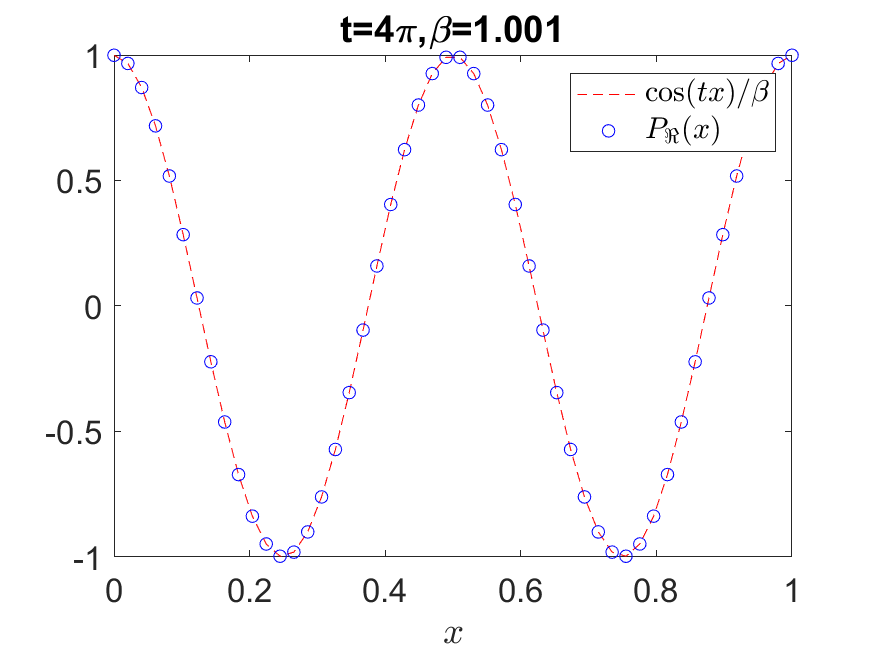
\includegraphics[width=0.31\textwidth]{HS_maxorder24_func}
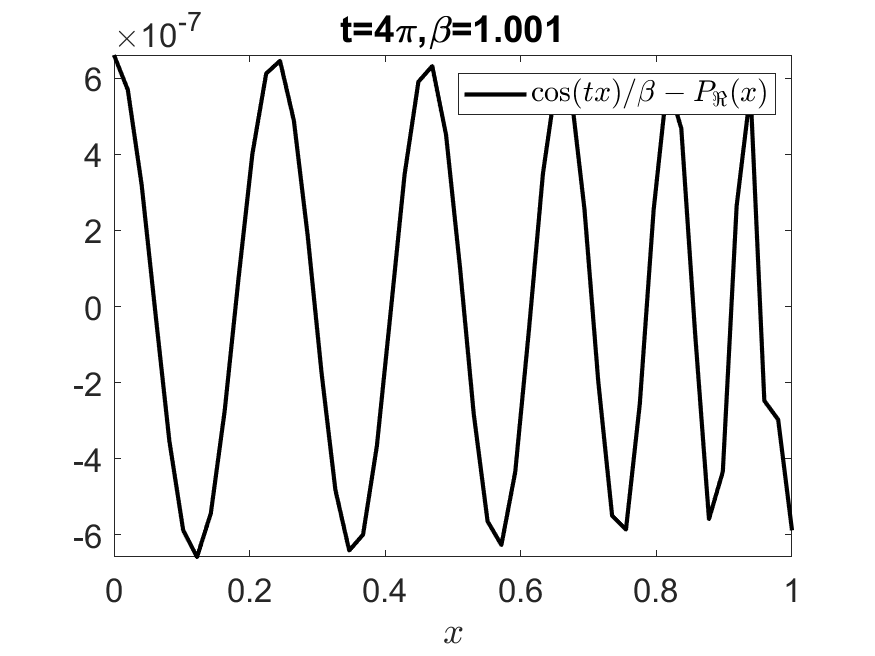
\includegraphics[width=0.31\textwidth]{HS_maxorder24_diff}
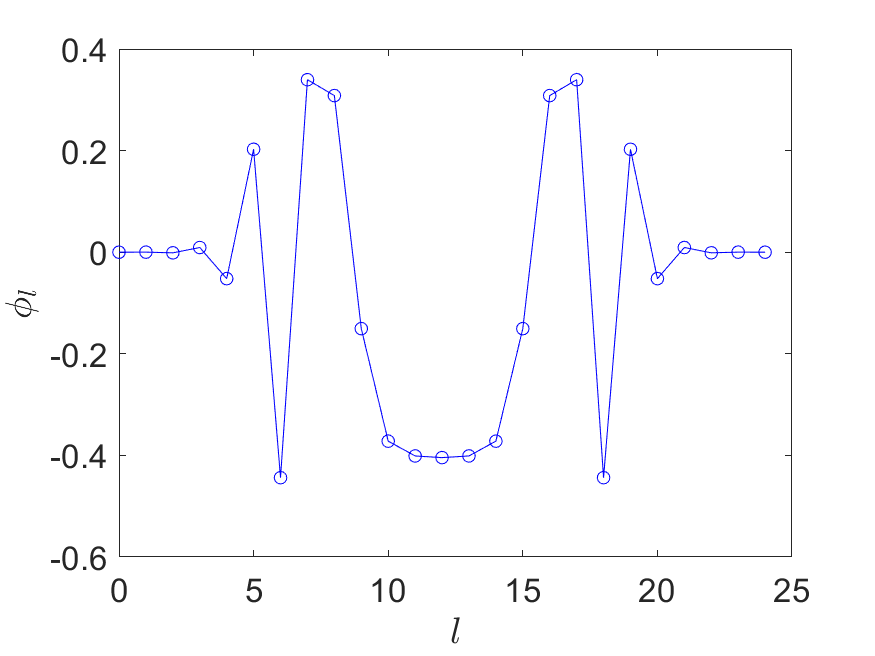
\includegraphics[width=0.31\textwidth]{HS_maxorder24_phase}
\end{center}
\caption{QSP representation of $\cos(tx)/\beta$ with $t=4\pi,\beta=1.001,d=24$. The phase factors plotted removes a factor of $\pi/4$ on both ends (see \cref{eqn:phi0}).}
\label{fig:qsp_HS_maxorder24}
\end{figure}

\begin{figure}[H]
\begin{center}
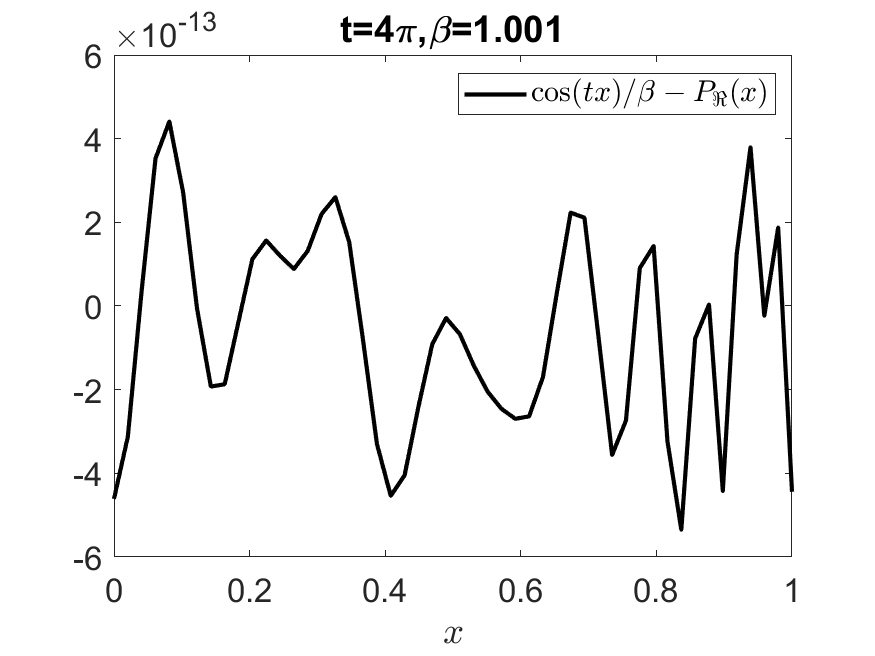
\includegraphics[width=0.4\textwidth]{HS_maxorder50_diff}
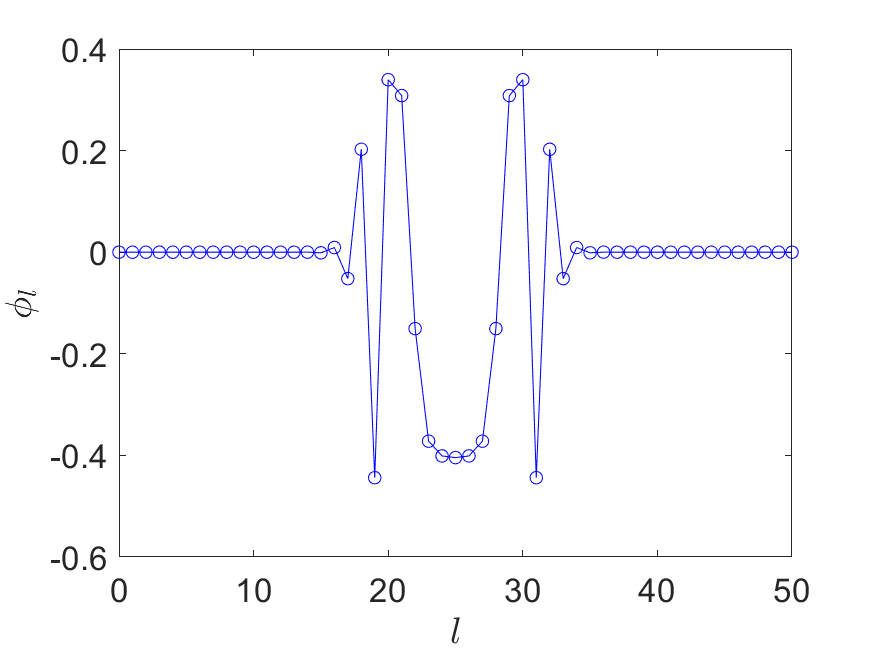
\includegraphics[width=0.4\textwidth]{HS_maxorder50_phase}
\end{center}
\caption{Error of the QSP representation of $\cos(tx)/\beta$ with $t=4\pi,\beta=1.001,d=50$. The phase factors plotted removes a factor of $\pi/4$ on both ends  (see \cref{eqn:phi0}).}
\label{fig:qsp_HS_maxorder50}
\end{figure}


\section{Application: Ground state preparation}\label{sec:qsp_groundstate}
%
Given a block encoding $U_H\in\BE_{1,m}(H)$, and WLOG assume $0\preceq H\preceq 1$. We assume that we are provided an initial state $\ket{\varphi}$ so that the initial overlap $p_0=\abs{\braket{\varphi|\psi_0}}^2$ is not small.
To simplify the problem we also assume that ground and the first excited state energies $E_0,E_1$ are known with a positive gap $\Delta:=E_1-E_0>0$. 
Our goal is to use QET to prepare an approximate quantum state $\ket{\psi}\approx \ket{\psi_0}$.

To this end, we can construct a threshold polynomial approximating the sign function on $[0,1]$. 
Due to the assumption that $0\preceq H\preceq 1$, this function can be chosen to be an even function. 
Since the sign function is a discontinuous, the polynomial should only aim at approximating the sign function outside $(\mu-\Delta/2,\mu+\Delta/2)$, where $\mu=(E_0+E_1)/2$. 
The polynomial also needs to satisfy the conditions in \cref{thm:qsp_real}.
We need to find an even polynomial $P_{\Re}(x)$ satisfying
\begin{equation}
\abs{P_{\Re}(x)-1}\le \epsilon, \quad \forall x\in [0,\mu-\Delta/2]; \quad \abs{P_{\Re}(x)}\le \epsilon, \quad \forall x\in [\mu+\Delta/2,1].
\end{equation}
We can achieve this by approximating the sign function, with $\deg(P_{\Re})=\Or(\log(1/\epsilon) \Delta^{-1})$. (see e.g.~\cite[Corollary 7]{LowChuang2017a} and \cite[Corollary 16]{GilyenSuLowEtAl2019}). 
This construction is based on an approximation to the $\mathrm{erf}$ function.
\cref{fig:qsp_step_deg80} gives a concrete construction of the even polynomial obtained via numerical optimization, and the phase factors are obtained via QSPPACK.


\begin{figure}[H]
\begin{center}
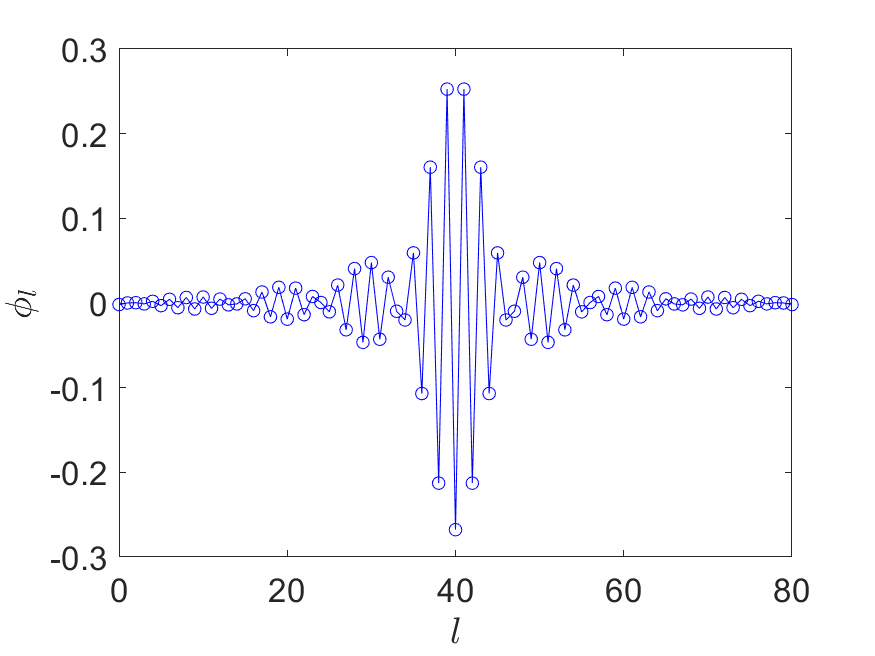
\includegraphics[width=0.31\textwidth]{step_deg80_phase}
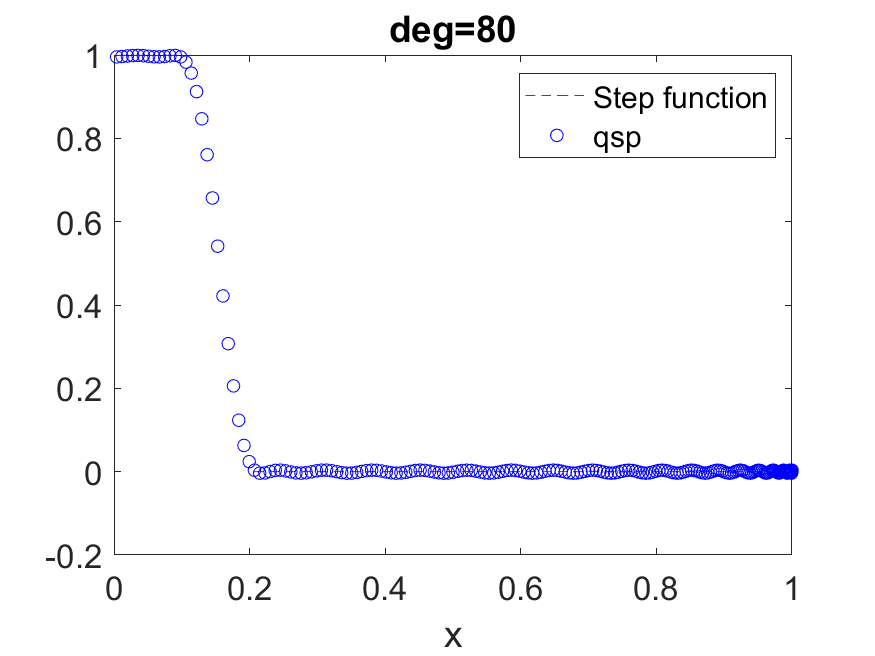
\includegraphics[width=0.31\textwidth]{step_deg80_func}
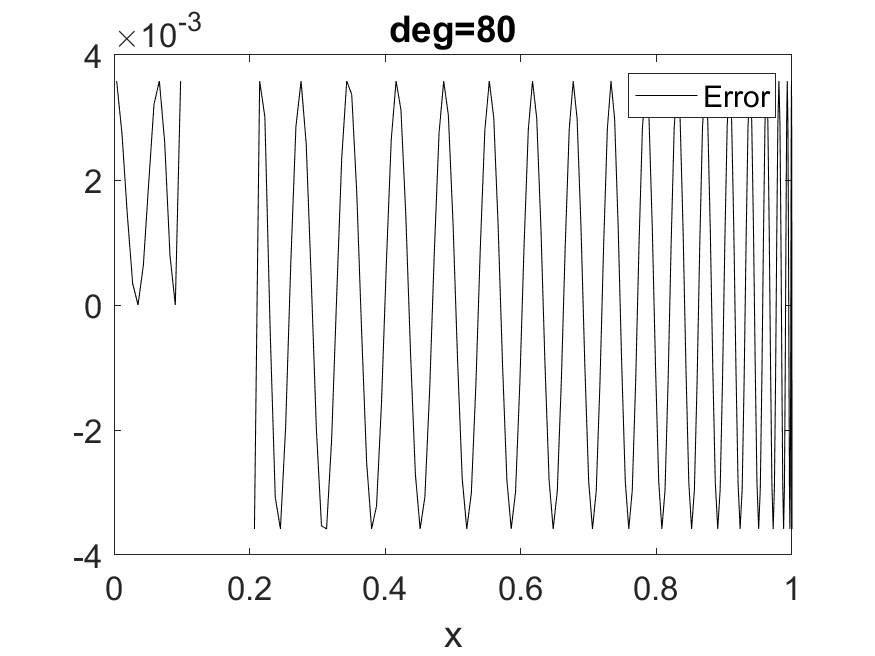
\includegraphics[width=0.31\textwidth]{step_deg80_diff}
\end{center}
\caption{QSP representation for approximating a step function using an even polynomial on $[0,0.1]\cup[0.2,1]$. The phase factors plotted removes a factor of $\pi/4$ on both ends (see \cref{eqn:phi0}).}
\label{fig:qsp_step_deg80}
\end{figure}


Applying the circuit $U_{\Phi}$ to the initial state $\ket{\varphi}$, we have
\begin{equation}
U_{\Phi}\ket{0^m}\ket{\varphi}=\sqrt{p_0} \ket{0^m} P_{\Re}(H) \ket{\psi_0}+\sqrt{1-p_0}\ket{0^m} P_{\Re}(H) \ket{\psi_{\perp}} + \ket{\perp}.
\end{equation}
Here $\ket{\psi_{\perp}}$ is a state in the system register orthogonal to $\ket{\psi_0}$, while $\ket{\perp}$ is orthogonal to all states $\ket{0^m}\ket{\psi}$. Note that 
\begin{equation}
\norm{P_{\Re}(H) \ket{\psi_{\perp}}}\le \epsilon, \quad \norm{P_{\Re}(H) \ket{\psi_0}}\ge 1-\epsilon,
\end{equation}
Therefore if we measure the ancilla qubits, the success probability of obtaining $0^m$ in the ancilla qubits, and the ground state $\ket{\psi_0}$ in the system register is at least $p_0 (1-\epsilon)$. So the total number of queries to to $U_A$ and $U_A^{\dag}$ is $\Or(\Delta^{-1}p_0^{-1}\log(1/\epsilon) )$.

Using amplitude amplification, the number of repetitions can be reduced to $\Or(\gamma^{-1})$, and the total number of queries to to $U_A$ and $U_A^{\dag}$ becomes $\Or(\Delta^{-1} p_0^{-\frac12}\log(1/\epsilon) )$. This also matches the lower bound~\cite{LinTong2020a}.

Once the ground state is prepared, we can estimate the ground state energy by measuring the expectation value $\braket{\psi_0|H|\psi_0}$. The number of samples needed is $\Or(1/\epsilon^2)$, which can be reduced to $\Or(1/\epsilon)$ using amplitude amplification. In summary, the best complexity for estimating the ground state energy $E_0$ to accuracy $\epsilon$ is $\Or(\Delta^{-1}p_0^{-\frac12}\epsilon^{-1}\log(1/\epsilon) )$. Note that the cost of estimating the ground state energy depends on the gap $\Delta$. 
This is because the algorithm first prepares the ground state and then estimates the ground state energy. 
If we are only interested in estimating $E_0$ to precision $\epsilon$, the gap dependence is not necessary (see~\cref{sec:groundenergy} as well as ~\cite{LinTong2020a}).



%\LL{Give examples and discuss the details later.} 
%
%
%Assume 
%Without loss of generality we assume , 
%Assume 
%Polynomial. QSPpack.


%\subsection{Quantum eigenvalue transformation viewed from the cosine-sine transformation*}



\vspace{2em}

\begin{exer}
Let $A,B$ be two $n$-qubit matrices. Construct a circuit to block encode $C=A+B$ with $U_A\in\BE_{\alpha_A,m}(A),U_B\in\BE_{\alpha_B,m}(B)$. 
\end{exer}

\begin{exer}
Use LCU to construct a block encoding of the TFIM model with periodic boundary conditions in \cref{eqn:ham_tfim}, with $g\ne 1$. 
\end{exer}

\begin{exer}
Prove \cref{prop:discriminant_reversiblewalk}.
\end{exer}


\begin{exer}
Let $A$ be an $n$-qubit Hermitian matrix. 
Write down the circuit for $U_{P_{\Re}(A)}\in\BE_{1,m+1}(P_{\Re}(A))$ with a block encoding $U_A\in\BE_{1,m}(A)$, where $P$ is characterized by the phase sequence $\wt{\Phi}$ specified in \cref{thm:qsp_simple}.
\end{exer}

\begin{exer}
Write down the circuit for LCU of Hamiltonian simulation.
\end{exer}

\begin{exer}
Using QET to prepare the Gibbs state.
\end{exer}
